\documentclass[twoside,a4paper,openany,12pt]{book}
\usepackage{amsfonts}
%% Disable ligatures in tt fonts, because we want to stop "--" being converted
%% to an en dash.
\usepackage{microtype}
\DisableLigatures[-]{family=tt*}

%%\documentclass[twoside,a4paper,12pt]{article}
%\documentclass[twoside,a4paper,openany,12pt]{report}

%% Document has convention that only first letter of chapters,
%% sections is capitalized. Do the same for automatic sections
\renewcommand\listfigurename{List of figures}
\renewcommand\listtablename{List of tables}
\newcommand{\secname}{Section}

%% Convenient way to specify margins
\usepackage[a4paper,top=2.5cm,bottom=2.5cm,inner=2.5cm,outer=2.5cm]{geometry}

%% Relative font sizes
\usepackage{relsize}

%% Use font with 8-bit encoding
\usepackage[T1]{fontenc}

%% Nicer fonts
\usepackage{pslatex}

\usepackage{linegoal}

%% Color definitions
\usepackage{color}
\definecolor{MyLightRed}{rgb}{1,.8,.8}
\definecolor{MyCodeboxColor}{rgb}{.9,.9,.9}
\definecolor{MyLightBlue}{rgb}{.8,.8,1}
\definecolor{MyQuoteColor}{rgb}{0,.6,0}
\definecolor{MyLightMagenta}{rgb}{1,.2,1}
\definecolor{MyYellow}{rgb}{1,1,.6}

%% For landscape pages printed, but rotated on screen
\usepackage{pdflscape}

%% Allow linebreaks in all captions. Required by the \photoCredit
%% command.
\usepackage{caption}
% \captionsetup{justification=justified}

%% Including figures and other graphics
\usepackage{graphicx}
% \usepackage[rgb]{xcolor}
%% Rotated images etc
\usepackage{rotating}

%% Author-year citations
\usepackage[authoryear]{natbib}

%% Subfigure environment
\usepackage{subfigure}

%% Conditional sections
\usepackage{ifthen}
\newcommand{\ifIsInstrument}[2]{\ifthenelse{\equal{\instrumentType}{#1}}{#2}{}}
\newcommand{\ifIsNotInstrument}[2]{\ifthenelse{\equal{\instrumentType}{#1}}{}{#2}}

\usepackage{etoolbox}

%% URLs
\usepackage[obeyspaces]{url}

%% SI units
\usepackage[abbreviations,binary-units=true]{siunitx}

% Command to get a tilde which prints as an ASCII tilde in PDFs,
% needed to allow copying text and pasting into a command window or
% editor
\newcommand{\mytilde}{\texttildelow}

%% For tables align on decimal point
\usepackage{dcolumn}
\newcolumntype{d}{D{.}{.}{-1}} % centre on decimal place

%% Long tables
\usepackage{supertabular}

\usepackage{fancyhdr}

%% Alternative to verbatim. Can be used for defining new environments
\usepackage{fancyvrb}
%% A command to include Matlab files (verbatim). Surrounded with a
%% frame and smaller font size than normal. Must be defined before
%% underscore package because the custom command must be listed in
%% \UnderscoreCommands
\CustomVerbatimCommand{\IncludeMatlabFileVerb}{VerbatimInput}{frame=single,fontsize=\relsize{-1}}
\CustomVerbatimCommand{\IncludeShellFileVerb}{VerbatimInput}{%
  frame=single,framesep=5mm,commandchars=\\\{\}
}

%% Include Matlab file verbatim and attach it for the user to download.
\newcommand{\IncludeMatlabFile}[2]{\IncludeMatlabFileVerb{#1}%
  \attachfile[mimetype=text/plain,description=#2]{#1}}

%% Include shell file verbatim and attach it for the user to download.
\newcommand{\IncludeShellFile}[2]{\IncludeShellFileVerb{#1}%
  \attachfile[mimetype=text/plain,description=#2]{#1}}


%% Have floats on subsequent page, not miles away.
\usepackage{flafter}

\usepackage{marvosym} % for \Info
\usepackage{keystroke} % for keyboard symbols

\usepackage{abbrev}
\renewcommand{\abbrevname}{Abbreviations}
%% List of abbreviations. Include all useful ones. Those which are not
%% used are not included in the table.

\abbrev{\adc}{ADC}{analogue to digital converter}
\abbrev{\cpu}{CPU}{central processing unit}
\abbrev{\dhcp}{DHCP}{dynamic host configuration protocol}
\abbrev{\dns}{DNS}{domain name system}
\abbrev{\esd}{ESD}{electro-static discharge}
\abbrev{\fet}{FET}{field-effect transistor}
\abbrev{\gpu}{GPU}{graphics processing unit}
\abbrev{\gui}{GUI}{graphical user interface}
\abbrev{\isp}{ISP}{in-circuit serial programmer (sometimes abbreviated
  as ICSP)}
\abbrev{\ip}{IP}{internet protocol}
\abbrev{\led}{LED}{light emitting diode}
\abbrev{\ntp}{NTP}{network time protocol}
\abbrev{\ota}{OTA}{over the air (as in firmware updates)}
\abbrev{\pcb}{PCB}{printed circuit board}
\abbrev{\psu}{PSU}{power supply unit}
\abbrev{\rfi}{RFI}{radio-frequency interference}
\abbrev{\rtc}{RTC}{real-time clock}
\abbrev{\sd}{SD}{secure digital}
\abbrev{\ssh}{SSH}{secure shell}
\abbrev{\samnet}{SAMNET}{Sub-Auroral Magnetometer Network}
\abbrev{\ttl}{TTL}{transistor-transistor logic}
\abbrev{\usb}{USB}{universal serial bus}
\abbrev{\ut}{UT}{universal time}
\abbrev{\utc}{UTC}{coordinated universal time}

\input{gitlog}

% Load the underscore package as fixes the problem of copying and
% pasting text with underscores; previously underscores were converted
% to spaces, but they matter for code! Need to protect certain
% commands which take input which has underscores (see underscore
% package for details)
\newcommand{\UnderscoreCommands}{%
  \do\VerbatimInput
  \do\BVerbatimInput
  \do\IncludeMatlabFileVerb
  \do\IncludeShellFileVerb
}
\usepackage[strings]{underscore}

\usepackage[%
bookmarksnumbered=true,
bookmarksopen=true,
bookmarksopenlevel=0,
unicode=true,colorlinks=false,
allbordercolors={0 0 1},
pdfborderstyle={/S/U/W 1}]{hyperref}

%% Have references to figures link to the top of the figure, not the
%% caption text.
\usepackage[all]{hypcap}

% Flush all floats at the start of a section
\usepackage[section]{placeins}
\usepackage{afterpage}

%% Attach files to PDF document. Set the default options we want.
\usepackage{attachfile2}
\attachfilesetup{icon=Paperclip}

%% Upright quotes, essential for quoting for Matlab code!
\usepackage{upquote}

\usepackage{pdfcomment}
\renewcommand{\insertabbrev}[2]{\pdftooltip{#1}{#2}}
\makeabbrev

%% A command for the return key
\newcommand{\myreturn}{%
  \keystroke{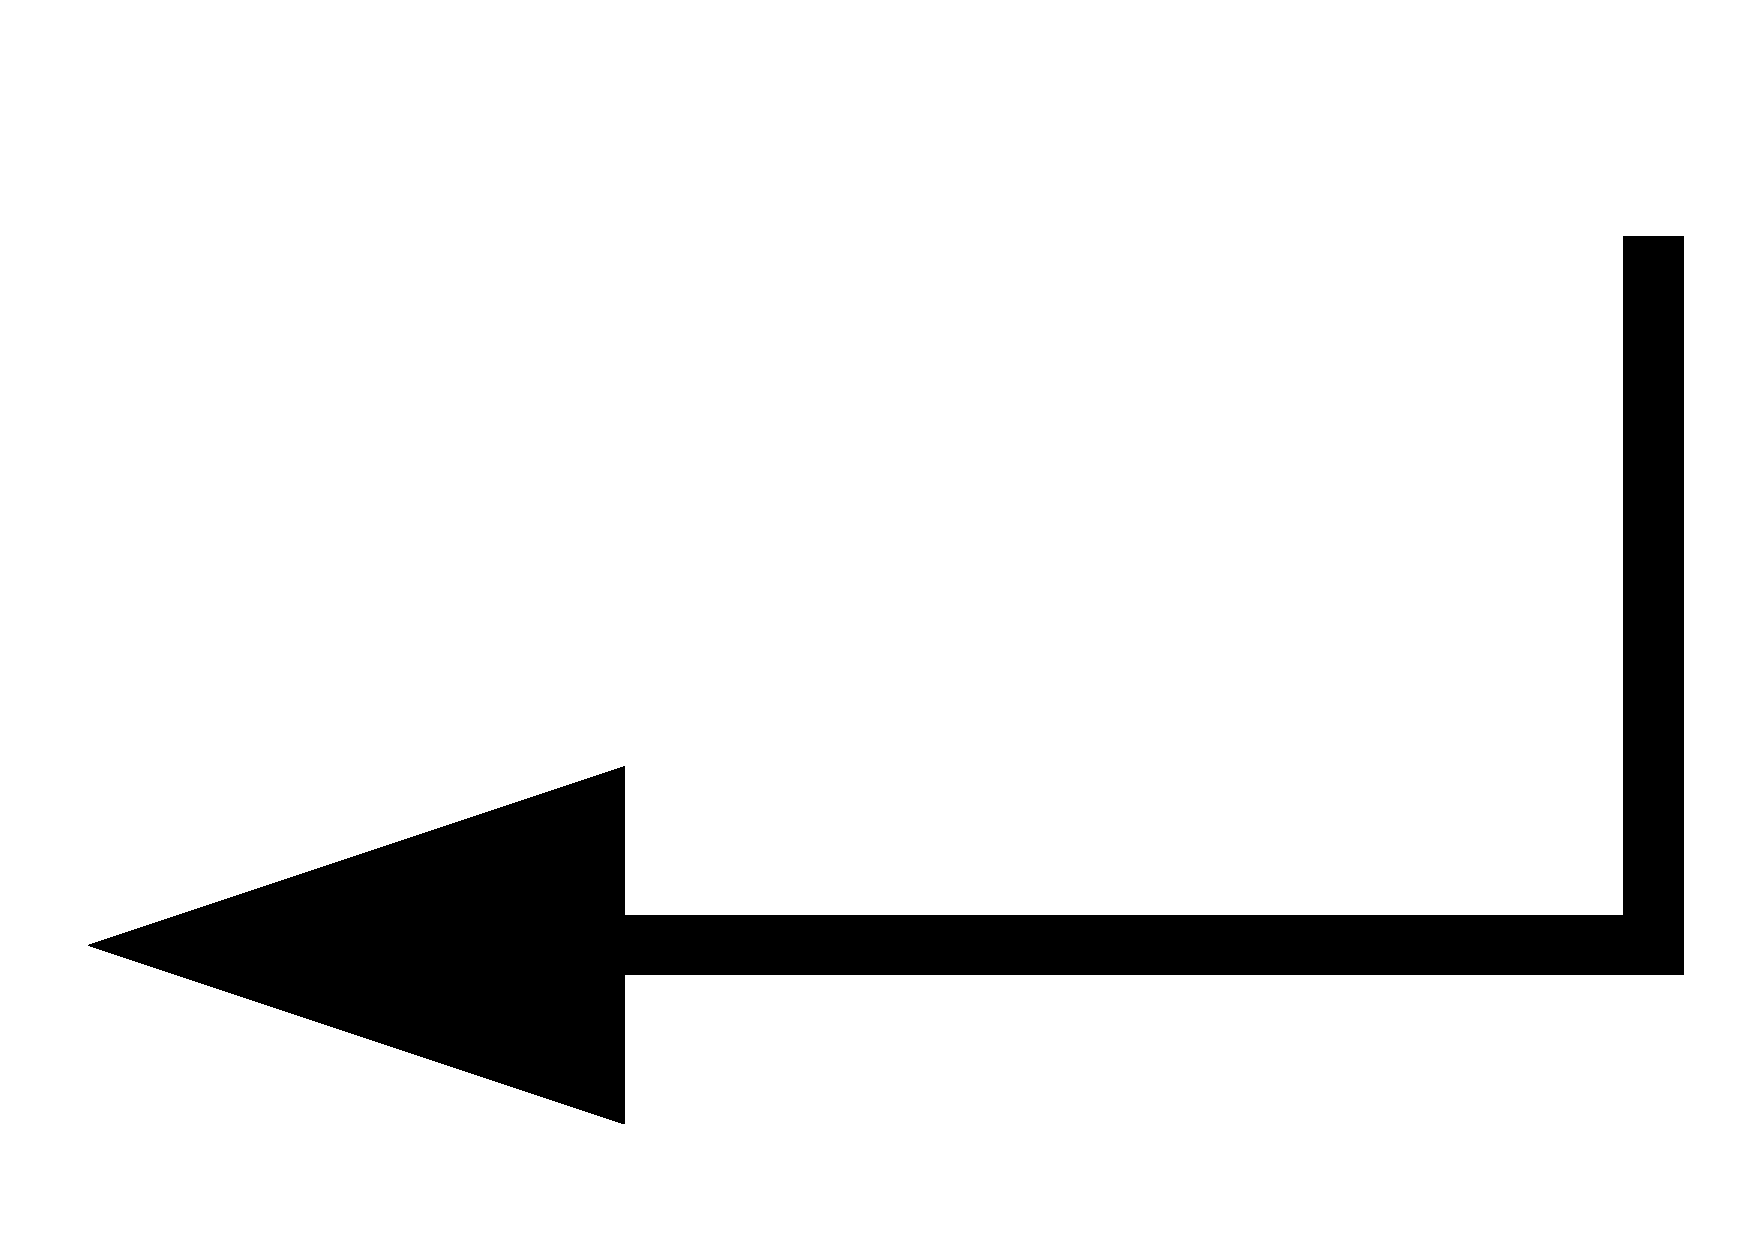
\includegraphics[width=1em]{images/return-symbol}}}

%% Change how subfigures are labelled
\makeatletter
\renewcommand{\@thesubfigure}{\figurename~\thefigure\alph{subfigure}: }
\renewcommand{\thesubfigure}{\alph{subfigure}}
%%%\renewcommand{\p@subfigure}{\alph{subfigure}}
\makeatother

% No indents at start of paragraph, but paragraphs have blank lines
% between them
\setlength{\parindent}{0pt}
\setlength{\parskip}{2ex} 


%% \filename allows for _ but otherwise is formatted identically to
%% code. If using tildes (~) then use \mytilde command, inside
%% \texttt. Use the url package's command to define this, that way
%% hyperref doesn't see it as a hyperref!
\DeclareUrlCommand\filename{\urlstyle{tt}}
\newcommand{\email}[1]{\href{mailto:#1}{#1}}
\newcommand{\ccBySaTwoUrl}{http://creativecommons.org/licenses/by-sa/2.0/}
\newcommand{\ccBySaThreeUrl}{http://creativecommons.org/licenses/by-sa/3.0/}

\newcommand{\ccBySaFourUrl}{http://creativecommons.org/licenses/by-sa/4.0/}
\newcommand{\ccByNcSaFourUrl}{%
  http://creativecommons.org/licenses/by-nc-sa/4.0/}

\newcommand{\ccBySaTwo}{\href{\ccBySaTwoUrl}{CC BY-SA 2.0}}
\newcommand{\ccBySaThree}{\href{\ccBySaThreeUrl}{CC BY-SA 3.0}}

\newcommand{\ccBySaFour}{\href{\ccBySaFourUrl}{CC BY-SA 4.0}}
\newcommand{\ccByNcSaFour}{\href{\ccByNcSaFourUrl}{CC BY-NC-SA 4.0}}

\newcommand{\rsyncUrl}{http://rsync.samba.org/}
%% Copyright, licence, URL.
\newcommand{\photoCredit}[4][]{\\ %
  \ifthenelse{\equal{#2}{}}{}{ \copyright~#2.}%
  \ifthenelse{\equal{#3}{}}{}{ #3.}%
  \ifthenelse{\equal{#4}{}}{}{ \href{#4}{#4}}}

%% Environment variables. Like \filename but prepends a $
\DeclareUrlCommand\envVar{\def\UrlLeft{\$}\urlstyle{tt}}
\DeclareUrlCommand\dosEnvVar{\def\UrlLeft{\%}\def\UrlRight{\%}\urlstyle{tt}}

\newcommand{\code}[1]{\texttt{#1}}
\newcommand{\username}[1]{\texttt{#1}}
\newcommand{\piUser}{\username{pi}}
\newcommand{\rootUser}{\username{root}}

%% Use for menu selections etc
\newcommand{\myquote}[1]{\textcolor{MyQuoteColor}{\textsl{#1}}}

%% Define our own keypress command, based on keystroke
\newcommand{\keypress}[1]{\keystroke{#1}}

%% Units
%%\newcommand{\units}[2]{\mbox{\ensuremath{#1}\,#2}}
%%\newcommand{\dB}[1]{\mbox{\ensuremath{#1}\,dB}}
\newcommand{\dB}[1]{\SI{#1}{dB}}
%%\newcommand{\inch}[1]{\mbox{\ensuremath{#1}''}}
\newcommand{\inch}[1]{\SI{#1}{''}}
\newcommand{\Hz}[1]{\SI{#1}{\hertz}}
\newcommand{\kHz}[1]{\SI{#1}{\kilo\hertz}}
\newcommand{\MHz}[1]{\SI{#1}{\mega\hertz}}
\newcommand{\volt}[1]{\SI{#1}{V}}
  \newcommand{\voltOLD}[1]{\mbox{\ensuremath{#1}\,V}}
\newcommand{\bit}[1]{\mbox{\ensuremath{#1}\,bit}}

%%\newcommand{\degrees}[1]{\ensuremath{#1^\circ}}
\newcommand{\degC}[1]{\ensuremath{#1^\circ}C}

\renewcommand{\textohm}{\ensuremath{\Omega}}
\newcommand{\ohm}[1]{\SI{#1}{\ohm}}
\newcommand{\kohm}[1]{\SI{#1}{\kilo\ohm}}
\newcommand{\Mohm}[1]{\SI{#1}{\mega\ohm}}


\newcommand{\pF}[1]{\SI{#1}{\pico\farad}}
\newcommand{\nF}[1]{\SI{#1}{\nano\farad}}
\newcommand{\uF}[1]{\SI{#1}{\micro\farad}}

\newcommand{\uH}[1]{\SI{#1}{\micro\henry}}

\newcommand{\nT}[1]{\SI{#1}{\nano\tesla}}

\newcommand{\MB}[1]{\SI{#1}{\mebi\byte}}

%% Some simple abbreviations  
\newcommand{\ie}{i.e.}
\newcommand{\eg}{e.g.}
\newcommand{\etal}{\latin{et al.}}
\newcommand{\etc}{etc.}

%% Have warnings printed in light red box, with each item using a
%% STOP sign as a bullet
\newenvironment{warninglist}{%
  \begin{list}{\Stopsign}{}}{%
    \end{list}}
\newcommand{\warningbox}[1]{\noindent\newline%
  \colorbox{MyLightRed}{\parbox{\textwidth}{%
      \begin{warninglist}\item #1\end{warninglist}}} \newline}

%% Have help information printed in light blue box, with each item using an
%% information sign as a bullet
\newenvironment{helplist}{%
  \begin{list}{\Info}{}}{%
    \end{list}}
\newcommand{\helpbox}[1]{\noindent\newline%
  \colorbox{MyLightBlue}{\parbox[l]{\textwidth}{%
      \begin{helplist}\item #1\end{helplist}}} \newline}
\newcommand{\examplebox}[2][]{\noindent\newline%
  \colorbox{MyYellow}{\parbox[l]{\textwidth}{\ifthenelse{\equal{#1}{}}%
      {Example: }{#1}\vspace*{1ex} \newline %
      #2 %
      \vspace*{1ex}}} \newline}


%% Verbatim-like environment for code.
\DefineVerbatimEnvironment{Code}{Verbatim}{%
  frame=single,commandchars=\\\{\}
}
\DefineVerbatimEnvironment{Cmd}{Verbatim}{%
  frame=single,framesep=5mm,commandchars=\\\{\}
}
\DefineVerbatimEnvironment{LinuxCmd}{Verbatim}{%
  frame=single,framesep=5mm,commandchars=\\\{\}
}
% {frame=single,label=\linuxLogo,framesep=5mm,commandchars=\\\{\}}
\DefineVerbatimEnvironment{WindowsCmd}{Verbatim}{%
  frame=single,framesep=5mm,commandchars=\\\{\}
}

\DefineVerbatimEnvironment{RootCmd}{Verbatim}%
{frame=single,framesep=5mm,label=As user \rootUser,commandchars=\\\{\}}
\DefineVerbatimEnvironment{PiCmd}{Verbatim}%
{frame=single,framesep=5mm,label=As user \piUser,commandchars=\\\{\}}


\newcommand{\todo}[1][]{\fcolorbox{magenta}{MyLightMagenta}{\mbox{\textcolor{black}{TO DO\ifthenelse{\equal{#1}{}}{}{: #1}}}}}

\newcommand{\figscale}{1.0}

%% Have subsubsections numbered
\setcounter{secnumdepth}{5}
\setcounter{tocdepth}{5}


\newenvironment{buildorder}{%
  \begin{enumerate}%
    \setlength{\itemsep}{0pt}%
    \setlength{\parskip}{0pt}}%
  {\end{enumerate}}
\newcounter{buildordercounter}
\newenvironment{buildorder*}{%
  \setcounter{buildordercounter}{\value{enumi}}
  \begin{enumerate}%
    \setcounter{enumi}{\value{buildordercounter}}
    \setlength{\itemsep}{0pt}%
    \setlength{\parskip}{0pt}}%
  {\end{enumerate}}

%\newenvironment{buildorder}{%
%  \begin{enumerate}[itemsep=0pt,parskip=0pt]}{\end{enumerate}}
% \newenvironment{buildorder*}{%
%   \begin{enumerate}[itemsep=0pt,parskip=0pt,resume*]}{\end{enumerate}}

\newcommand{\copyrightyear}{%
  \ifthenelse{\equal{\gitCommitYear}{2014}}{2014}{2014--\gitCommitYear}
}
\newcommand{\documentAttribution}{%
\ifthenelse{\equal{\instrumentType}{magnetometer}}{%
``AuroraWatchNet magnetometer manual. Steve R. Marple. \gitCommitYear.''}{%
``Riometer manual. Steve R. Marple. \gitCommitYear.''}}

\typeout{Job is \jobname}
\expandafter\ifstrequal\expandafter{\jobname}{calunium-mag-manual}{%
  \typeout{Making Calunium manual}%
  \def\caluniumMagManual{}
  \def\instrumentType{magnetometer}
  \def\usesMicrocontroller{}
}{%
  \typeout{Not Calunium manual!}
}
\expandafter\ifstrequal\expandafter{\jobname}{raspi-mag-manual}{%
  \typeout{Making AuroraWatchNet Raspberry Pi manual}%
  \def\raspiMagManual{}
  \def\instrumentType{magnetometer}
}{%
  \typeout{Not AuroraWatchNet Raspberry Pi manual!}
}
\expandafter\ifstrequal\expandafter{\jobname}{bgs-mag-manual}{%
  \typeout{Making BGS Raspberry Pi manual}%
  \def\bgsMagManual{}
  \def\instrumentType{magnetometer}
}{%
  \typeout{Not BGS Raspberry Pi manual!}
}
\expandafter\ifstrequal\expandafter{\jobname}{riometer-manual}{%
  \typeout{Making riometer manual}%
  \def\riometerManual{}
  \def\instrumentType{riometer}
  \def\usesMicrocontroller{}
}{%
  \typeout{Not riometer manual!}
}


\begin{document}

\ifdef{\caluniumMagManual}{%
  \title{AuroraWatchNet magnetometer manual\newline
  \large For PoE and radio systems using Calunium microcontroller}%
}{}
\ifdef{\raspiMagManual}{%
  \title{AuroraWatchNet Raspberry Pi\\
    magnetometer manual}%
}{}
\ifdef{\bgsMagManual}{%
  \title{BGS Raspberry Pi magnetometer\\
  \Large Software configuration and operation manual}%
}{}
\ifdef{\riometerManual}{%
  \title{Riometer manual\\
  \Large Software configuration and operation manual}%
}{}
\author{Steve R. Marple, \\
Lancaster University.}
\date{\gitCommitDate\\
  \small{Commit: \gitCommit}}
\maketitle
\thispagestyle{empty}
\frontmatter
\pagestyle{headings}

% \clearpage  
% \phantomsection  
% % \thispagestyle{empty}
\chapter{Licence}
This document is made available under the \href{\ccBySaFourUrl}{Creative
  Commons Attribution-ShareAlike 4.0 Unported Licence}.

\begin{center}
\href{\ccBySaFourUrl}{\includegraphics{images/by-sa}}
\end{center}

Please attribute this work as \documentAttribution

\clearpage  
\phantomsection  
\addcontentsline{toc}{chapter}{\contentsname}  
\tableofcontents

\newpage
\phantomsection  
\addcontentsline{toc}{chapter}{\listfigurename}  
\listoffigures

%% -----------------------------
% \newpage
% \phantomsection  
% \addcontentsline{toc}{chapter}{\listtablename}  
% \listoftables

\newpage
\phantomsection  
\printabbrev

\mainmatter
%% Allow for sloppy wordbreaking to avoid text spilling into the
%% margin (eg as a result of \filename and other non-breaking text)
\sloppy

%%%%%%%%%%%%%%%%%%%%%%%%%%%%%%%%%%%%%%%%%%%%%%%%%%%%%%%%%%%%%%%
%%%
%%% INTRODUCTION
%%%
%%%%%%%%%%%%%%%%%%%%%%%%%%%%%%%%%%%%%%%%%%%%%%%%%%%%%%%%%%%%%%%
 \part{Introduction}
\ifdef{\caluniumMagManual}{%
  \chapter{Overview of the hardware}

\section{Introduction}

The riometer data logger is an extension of the AuroraWatchNet
project, an open-source magnetometer designed for generating real-time
alerts when aurora might be visible by lower-latitude observers. The
magnetometer was originally designed with a battery-powered remote
sensor unit that was located outdoors and away from human
disturbance. It connected via a radio link to a base unit indoors that
contained a Raspberry Pi single board computer. Later a power over
Ethernet (\PoE) remote sensor unit was designed. The hardware and
software have had extensive testing and operation since the project's
inception in 2012.

In the riometer data logger all of the electronics are located
indoors. For convenience the sensor unit and Raspberry Pi are
contained in the same enclosure. For single-beam riometer systems the
riometer is also contained in the same enclosure. For imaging riometer
systems the riometers and Butler matrix units are contained in their
own enclosures.

\section{Hardware description}

The sensor unit of the riometer data logger makes uses of the existing
Power over Ethernet microcontroller board. It is itself a derivation
of the Calunium project by the author to create an Atmel ATmega1284P
Arduino clone. The benefit of the ATmega1284P is the larger memory
available compared to most Arduino boards, yet still retains the
convenience of a through-hole package for easy home assembly and
tool-less replacement during servicing.

All of the data acquisition, timing, temporary storage, collection of
house-keeping data and transmission over Ethernet is performed by an
Atmel ATmega1284P microcontroller running at \MHz{20}. The firmware
was developed using the Arduino development environment. This was
chosen at the beginning of the AuroraWatchNet project to foster an
open environment conducive to collaboration. Many of the software
modules used to support the data logger were written specifically for
the project and have been released as independent open source
software. Most of the software modules implement their own state
machines to allow efficient and cooperative real time
operation. Remote over the air firmware updates are made possible by
the xboot bootloader; updates via the \usb\ interface are also
supported.

Analogue signals are converted to digital values by one or more
Microchip MCP3424 analogue to digital converters (one for wide beam
riometer systems, for imaging riometers each image column has its own
\adc). In the case of multiple \adc s they are simultaneously
commanded to being sampling. The microcontroller is responsible for
initiating data sampling, using its internal software real time clock
or a \gnss\ pulse-per-second signal. If over-sampling has been
selected the samples are reduced to a single value for each beam. The
resulting samples for each beam are stored in a buffer for subsequent
transmission over Ethernet to a Python data logger daemon running on a
Raspberry Pi.

The Ethernet interface uses a standard Arduino Ethernet shield. Either
the older Wiznet W5100 model or the newer Wiznet W5500 model can be
used but the correct firmware version must be programmed into the
microcontroller.


\section{Clock sources}

The sensor unit has a number of clock sources available and will use
the best source available to timestamp the data. The timestamp
corresponds to the beginning of the data sampling period (not
necessarily the exact moment data sampling began as there may be a
pre-sample delay configured). The clock sources are:
\begin{itemize}
\item The onboard real time clock \ic. The clock runs from a
  \Hz{32768} watch crystal with a typical accuracy of
  \SI{20}{ppm}. The time can only be read back with a precision of one
  second.
\item The \gnss\ combined clock source. When multiple satellite
  constellations are in use the \gnss\ module derives its time and
  location fix from all of the suitable satellites in view. Clock
  accuracy is excellent, the pulse-per-second output has an accuracy
  of \SI{\pm15}{\nano\second} (requires the correct antenna delay
  compensation for this accuracy to be achieved). Requires the
  firmware to be compiled with \code{FEATURE_GNSS} enabled.
\item The server clock, obtained from the acknowledgement message. The
  server clock time is sent only when the Raspberry Pi \ntp\ service
  has a valid time.
\end{itemize}

To manage these different clock sources the microcontroller implements
a software real time clock module. On start up the clock is
initialized from the onboard real time clock \ic, with the limitation
that the precision is limited to one second. However the software
clock uses the \Hz{32768} square wave output to achieve higher
internal resolution.

When the server clock time is available it is compared to the internal
software clock, and if necessary the software clock is adjusted. Time
adjustments are limited to when the difference is deemed too large, to
avoid adding unnecessary clock jitter to the acquired data samples.

When the \gnss\ module has a valid position and time fix its next
pulse-per-second output is used to set the internal software
clock. Data acquisition commences immediately on receipt of a valid
pulse-per-second edge, or if one is not available at the next
prescribed sampling time using the internal software clock. Thus when
the \gnss\ module has a valid fix data timestamps are placed at the
second boundary, otherwise they will occur (to best effort) at $n$
second intervals where $n$ is the sampling interval in seconds but not
necessarily on a second boundary.

The hardware real time clock \ic\ is set periodically to ensure
accurate time-keeping from a cold-start when the Raspberry Pi does not
have a valid time from \ntp\ and before the \gnss\ module has been
able to acquire a position and time fix.

\helpbox{%
  The server time clock is never used for time-keeping whilst the
  \gnss\ module has a valid position and time fix.
\item The \gnss\ position, time and satellites in view information are
  reported with the next data sample. Thus when monitoring the serial
  console or \gnss\ data files it may appear that this information is
  sent late. The microcontroller firmware uses the current \gnss\ time
  to compute the time for the next pulse-per-per second signal to
  ensure the correct data stamps are applied to the data. This can be
  confirmed by monitoring a \gnss\ clock or the time at
  \url{https://time.is/} and comparing with the incoming data
  timestamps.}

}{}
\ifdef{\raspiMagManual}{%
  \chapter{Overview of the hardware}

\section{Introduction}

The riometer data logger is an extension of the AuroraWatchNet
project, an open-source magnetometer designed for generating real-time
alerts when aurora might be visible by lower-latitude observers. The
magnetometer was originally designed with a battery-powered remote
sensor unit that was located outdoors and away from human
disturbance. It connected via a radio link to a base unit indoors that
contained a Raspberry Pi single board computer. Later a power over
Ethernet (\PoE) remote sensor unit was designed. The hardware and
software have had extensive testing and operation since the project's
inception in 2012.

In the riometer data logger all of the electronics are located
indoors. For convenience the sensor unit and Raspberry Pi are
contained in the same enclosure. For single-beam riometer systems the
riometer is also contained in the same enclosure. For imaging riometer
systems the riometers and Butler matrix units are contained in their
own enclosures.

\section{Hardware description}

The sensor unit of the riometer data logger makes uses of the existing
Power over Ethernet microcontroller board. It is itself a derivation
of the Calunium project by the author to create an Atmel ATmega1284P
Arduino clone. The benefit of the ATmega1284P is the larger memory
available compared to most Arduino boards, yet still retains the
convenience of a through-hole package for easy home assembly and
tool-less replacement during servicing.

All of the data acquisition, timing, temporary storage, collection of
house-keeping data and transmission over Ethernet is performed by an
Atmel ATmega1284P microcontroller running at \MHz{20}. The firmware
was developed using the Arduino development environment. This was
chosen at the beginning of the AuroraWatchNet project to foster an
open environment conducive to collaboration. Many of the software
modules used to support the data logger were written specifically for
the project and have been released as independent open source
software. Most of the software modules implement their own state
machines to allow efficient and cooperative real time
operation. Remote over the air firmware updates are made possible by
the xboot bootloader; updates via the \usb\ interface are also
supported.

Analogue signals are converted to digital values by one or more
Microchip MCP3424 analogue to digital converters (one for wide beam
riometer systems, for imaging riometers each image column has its own
\adc). In the case of multiple \adc s they are simultaneously
commanded to being sampling. The microcontroller is responsible for
initiating data sampling, using its internal software real time clock
or a \gnss\ pulse-per-second signal. If over-sampling has been
selected the samples are reduced to a single value for each beam. The
resulting samples for each beam are stored in a buffer for subsequent
transmission over Ethernet to a Python data logger daemon running on a
Raspberry Pi.

The Ethernet interface uses a standard Arduino Ethernet shield. Either
the older Wiznet W5100 model or the newer Wiznet W5500 model can be
used but the correct firmware version must be programmed into the
microcontroller.


\section{Clock sources}

The sensor unit has a number of clock sources available and will use
the best source available to timestamp the data. The timestamp
corresponds to the beginning of the data sampling period (not
necessarily the exact moment data sampling began as there may be a
pre-sample delay configured). The clock sources are:
\begin{itemize}
\item The onboard real time clock \ic. The clock runs from a
  \Hz{32768} watch crystal with a typical accuracy of
  \SI{20}{ppm}. The time can only be read back with a precision of one
  second.
\item The \gnss\ combined clock source. When multiple satellite
  constellations are in use the \gnss\ module derives its time and
  location fix from all of the suitable satellites in view. Clock
  accuracy is excellent, the pulse-per-second output has an accuracy
  of \SI{\pm15}{\nano\second} (requires the correct antenna delay
  compensation for this accuracy to be achieved). Requires the
  firmware to be compiled with \code{FEATURE_GNSS} enabled.
\item The server clock, obtained from the acknowledgement message. The
  server clock time is sent only when the Raspberry Pi \ntp\ service
  has a valid time.
\end{itemize}

To manage these different clock sources the microcontroller implements
a software real time clock module. On start up the clock is
initialized from the onboard real time clock \ic, with the limitation
that the precision is limited to one second. However the software
clock uses the \Hz{32768} square wave output to achieve higher
internal resolution.

When the server clock time is available it is compared to the internal
software clock, and if necessary the software clock is adjusted. Time
adjustments are limited to when the difference is deemed too large, to
avoid adding unnecessary clock jitter to the acquired data samples.

When the \gnss\ module has a valid position and time fix its next
pulse-per-second output is used to set the internal software
clock. Data acquisition commences immediately on receipt of a valid
pulse-per-second edge, or if one is not available at the next
prescribed sampling time using the internal software clock. Thus when
the \gnss\ module has a valid fix data timestamps are placed at the
second boundary, otherwise they will occur (to best effort) at $n$
second intervals where $n$ is the sampling interval in seconds but not
necessarily on a second boundary.

The hardware real time clock \ic\ is set periodically to ensure
accurate time-keeping from a cold-start when the Raspberry Pi does not
have a valid time from \ntp\ and before the \gnss\ module has been
able to acquire a position and time fix.

\helpbox{%
  The server time clock is never used for time-keeping whilst the
  \gnss\ module has a valid position and time fix.
\item The \gnss\ position, time and satellites in view information are
  reported with the next data sample. Thus when monitoring the serial
  console or \gnss\ data files it may appear that this information is
  sent late. The microcontroller firmware uses the current \gnss\ time
  to compute the time for the next pulse-per-per second signal to
  ensure the correct data stamps are applied to the data. This can be
  confirmed by monitoring a \gnss\ clock or the time at
  \url{https://time.is/} and comparing with the incoming data
  timestamps.}

}{}
\ifdef{\bgsMagManual}{%
  \chapter{Overview of the hardware}

\section{Introduction}

The riometer data logger is an extension of the AuroraWatchNet
project, an open-source magnetometer designed for generating real-time
alerts when aurora might be visible by lower-latitude observers. The
magnetometer was originally designed with a battery-powered remote
sensor unit that was located outdoors and away from human
disturbance. It connected via a radio link to a base unit indoors that
contained a Raspberry Pi single board computer. Later a power over
Ethernet (\PoE) remote sensor unit was designed. The hardware and
software have had extensive testing and operation since the project's
inception in 2012.

In the riometer data logger all of the electronics are located
indoors. For convenience the sensor unit and Raspberry Pi are
contained in the same enclosure. For single-beam riometer systems the
riometer is also contained in the same enclosure. For imaging riometer
systems the riometers and Butler matrix units are contained in their
own enclosures.

\section{Hardware description}

The sensor unit of the riometer data logger makes uses of the existing
Power over Ethernet microcontroller board. It is itself a derivation
of the Calunium project by the author to create an Atmel ATmega1284P
Arduino clone. The benefit of the ATmega1284P is the larger memory
available compared to most Arduino boards, yet still retains the
convenience of a through-hole package for easy home assembly and
tool-less replacement during servicing.

All of the data acquisition, timing, temporary storage, collection of
house-keeping data and transmission over Ethernet is performed by an
Atmel ATmega1284P microcontroller running at \MHz{20}. The firmware
was developed using the Arduino development environment. This was
chosen at the beginning of the AuroraWatchNet project to foster an
open environment conducive to collaboration. Many of the software
modules used to support the data logger were written specifically for
the project and have been released as independent open source
software. Most of the software modules implement their own state
machines to allow efficient and cooperative real time
operation. Remote over the air firmware updates are made possible by
the xboot bootloader; updates via the \usb\ interface are also
supported.

Analogue signals are converted to digital values by one or more
Microchip MCP3424 analogue to digital converters (one for wide beam
riometer systems, for imaging riometers each image column has its own
\adc). In the case of multiple \adc s they are simultaneously
commanded to being sampling. The microcontroller is responsible for
initiating data sampling, using its internal software real time clock
or a \gnss\ pulse-per-second signal. If over-sampling has been
selected the samples are reduced to a single value for each beam. The
resulting samples for each beam are stored in a buffer for subsequent
transmission over Ethernet to a Python data logger daemon running on a
Raspberry Pi.

The Ethernet interface uses a standard Arduino Ethernet shield. Either
the older Wiznet W5100 model or the newer Wiznet W5500 model can be
used but the correct firmware version must be programmed into the
microcontroller.


\section{Clock sources}

The sensor unit has a number of clock sources available and will use
the best source available to timestamp the data. The timestamp
corresponds to the beginning of the data sampling period (not
necessarily the exact moment data sampling began as there may be a
pre-sample delay configured). The clock sources are:
\begin{itemize}
\item The onboard real time clock \ic. The clock runs from a
  \Hz{32768} watch crystal with a typical accuracy of
  \SI{20}{ppm}. The time can only be read back with a precision of one
  second.
\item The \gnss\ combined clock source. When multiple satellite
  constellations are in use the \gnss\ module derives its time and
  location fix from all of the suitable satellites in view. Clock
  accuracy is excellent, the pulse-per-second output has an accuracy
  of \SI{\pm15}{\nano\second} (requires the correct antenna delay
  compensation for this accuracy to be achieved). Requires the
  firmware to be compiled with \code{FEATURE_GNSS} enabled.
\item The server clock, obtained from the acknowledgement message. The
  server clock time is sent only when the Raspberry Pi \ntp\ service
  has a valid time.
\end{itemize}

To manage these different clock sources the microcontroller implements
a software real time clock module. On start up the clock is
initialized from the onboard real time clock \ic, with the limitation
that the precision is limited to one second. However the software
clock uses the \Hz{32768} square wave output to achieve higher
internal resolution.

When the server clock time is available it is compared to the internal
software clock, and if necessary the software clock is adjusted. Time
adjustments are limited to when the difference is deemed too large, to
avoid adding unnecessary clock jitter to the acquired data samples.

When the \gnss\ module has a valid position and time fix its next
pulse-per-second output is used to set the internal software
clock. Data acquisition commences immediately on receipt of a valid
pulse-per-second edge, or if one is not available at the next
prescribed sampling time using the internal software clock. Thus when
the \gnss\ module has a valid fix data timestamps are placed at the
second boundary, otherwise they will occur (to best effort) at $n$
second intervals where $n$ is the sampling interval in seconds but not
necessarily on a second boundary.

The hardware real time clock \ic\ is set periodically to ensure
accurate time-keeping from a cold-start when the Raspberry Pi does not
have a valid time from \ntp\ and before the \gnss\ module has been
able to acquire a position and time fix.

\helpbox{%
  The server time clock is never used for time-keeping whilst the
  \gnss\ module has a valid position and time fix.
\item The \gnss\ position, time and satellites in view information are
  reported with the next data sample. Thus when monitoring the serial
  console or \gnss\ data files it may appear that this information is
  sent late. The microcontroller firmware uses the current \gnss\ time
  to compute the time for the next pulse-per-per second signal to
  ensure the correct data stamps are applied to the data. This can be
  confirmed by monitoring a \gnss\ clock or the time at
  \url{https://time.is/} and comparing with the incoming data
  timestamps.}

}{}
\ifdef{\riometerManual}{%
  \chapter{Overview of the hardware}

\section{Introduction}

The riometer data logger is an extension of the AuroraWatchNet
project, an open-source magnetometer designed for generating real-time
alerts when aurora might be visible by lower-latitude observers. The
magnetometer was originally designed with a battery-powered remote
sensor unit that was located outdoors and away from human
disturbance. It connected via a radio link to a base unit indoors that
contained a Raspberry Pi single board computer. Later a power over
Ethernet (\PoE) remote sensor unit was designed. The hardware and
software have had extensive testing and operation since the project's
inception in 2012.

In the riometer data logger all of the electronics are located
indoors. For convenience the sensor unit and Raspberry Pi are
contained in the same enclosure. For single-beam riometer systems the
riometer is also contained in the same enclosure. For imaging riometer
systems the riometers and Butler matrix units are contained in their
own enclosures.

\section{Hardware description}

The sensor unit of the riometer data logger makes uses of the existing
Power over Ethernet microcontroller board. It is itself a derivation
of the Calunium project by the author to create an Atmel ATmega1284P
Arduino clone. The benefit of the ATmega1284P is the larger memory
available compared to most Arduino boards, yet still retains the
convenience of a through-hole package for easy home assembly and
tool-less replacement during servicing.

All of the data acquisition, timing, temporary storage, collection of
house-keeping data and transmission over Ethernet is performed by an
Atmel ATmega1284P microcontroller running at \MHz{20}. The firmware
was developed using the Arduino development environment. This was
chosen at the beginning of the AuroraWatchNet project to foster an
open environment conducive to collaboration. Many of the software
modules used to support the data logger were written specifically for
the project and have been released as independent open source
software. Most of the software modules implement their own state
machines to allow efficient and cooperative real time
operation. Remote over the air firmware updates are made possible by
the xboot bootloader; updates via the \usb\ interface are also
supported.

Analogue signals are converted to digital values by one or more
Microchip MCP3424 analogue to digital converters (one for wide beam
riometer systems, for imaging riometers each image column has its own
\adc). In the case of multiple \adc s they are simultaneously
commanded to being sampling. The microcontroller is responsible for
initiating data sampling, using its internal software real time clock
or a \gnss\ pulse-per-second signal. If over-sampling has been
selected the samples are reduced to a single value for each beam. The
resulting samples for each beam are stored in a buffer for subsequent
transmission over Ethernet to a Python data logger daemon running on a
Raspberry Pi.

The Ethernet interface uses a standard Arduino Ethernet shield. Either
the older Wiznet W5100 model or the newer Wiznet W5500 model can be
used but the correct firmware version must be programmed into the
microcontroller.


\section{Clock sources}

The sensor unit has a number of clock sources available and will use
the best source available to timestamp the data. The timestamp
corresponds to the beginning of the data sampling period (not
necessarily the exact moment data sampling began as there may be a
pre-sample delay configured). The clock sources are:
\begin{itemize}
\item The onboard real time clock \ic. The clock runs from a
  \Hz{32768} watch crystal with a typical accuracy of
  \SI{20}{ppm}. The time can only be read back with a precision of one
  second.
\item The \gnss\ combined clock source. When multiple satellite
  constellations are in use the \gnss\ module derives its time and
  location fix from all of the suitable satellites in view. Clock
  accuracy is excellent, the pulse-per-second output has an accuracy
  of \SI{\pm15}{\nano\second} (requires the correct antenna delay
  compensation for this accuracy to be achieved). Requires the
  firmware to be compiled with \code{FEATURE_GNSS} enabled.
\item The server clock, obtained from the acknowledgement message. The
  server clock time is sent only when the Raspberry Pi \ntp\ service
  has a valid time.
\end{itemize}

To manage these different clock sources the microcontroller implements
a software real time clock module. On start up the clock is
initialized from the onboard real time clock \ic, with the limitation
that the precision is limited to one second. However the software
clock uses the \Hz{32768} square wave output to achieve higher
internal resolution.

When the server clock time is available it is compared to the internal
software clock, and if necessary the software clock is adjusted. Time
adjustments are limited to when the difference is deemed too large, to
avoid adding unnecessary clock jitter to the acquired data samples.

When the \gnss\ module has a valid position and time fix its next
pulse-per-second output is used to set the internal software
clock. Data acquisition commences immediately on receipt of a valid
pulse-per-second edge, or if one is not available at the next
prescribed sampling time using the internal software clock. Thus when
the \gnss\ module has a valid fix data timestamps are placed at the
second boundary, otherwise they will occur (to best effort) at $n$
second intervals where $n$ is the sampling interval in seconds but not
necessarily on a second boundary.

The hardware real time clock \ic\ is set periodically to ensure
accurate time-keeping from a cold-start when the Raspberry Pi does not
have a valid time from \ntp\ and before the \gnss\ module has been
able to acquire a position and time fix.

\helpbox{%
  The server time clock is never used for time-keeping whilst the
  \gnss\ module has a valid position and time fix.
\item The \gnss\ position, time and satellites in view information are
  reported with the next data sample. Thus when monitoring the serial
  console or \gnss\ data files it may appear that this information is
  sent late. The microcontroller firmware uses the current \gnss\ time
  to compute the time for the next pulse-per-per second signal to
  ensure the correct data stamps are applied to the data. This can be
  confirmed by monitoring a \gnss\ clock or the time at
  \url{https://time.is/} and comparing with the incoming data
  timestamps.}

}{}

%%%%%%%%%%%%%%%%%%%%%%%%%%%%%%%%%%%%%%%%%%%%%%%%%%%%%%%%%%%%%%%
%%%
%%% CONSTRUCTION
%%%
%%% Note that there is no construction for the BGS mag - see BGS for
%%% information.
%%%
%%%%%%%%%%%%%%%%%%%%%%%%%%%%%%%%%%%%%%%%%%%%%%%%%%%%%%%%%%%%%%%
\ifdef{\caluniumMagManual}{%
  \part{Construction}
  \chapter{Beginning construction}

\section{Anti-static precautions}

\section{Tools required}

\begin{itemize}
\item Soldering iron.
\item Sidecutters.
\item Small pliers.
\item In-circuit serial programmer for Atmel AVR microcontrollers,
  \eg, \href{http://www.atmel.com/tools/AVRDRAGON.aspx}{Atmel AVR Dragon}.
\item USB to TTL serial converter for \volt{3.3} operation, \eg, FTDI
  TTL-232R-3V3.
\item Digital multimeter.
\item Solderless breadboard (optional).
\end{itemize}

\section{Order of assembly}

For ease of access components should normally be fitted in order of
increasing size, particularly increasing height. If this order is not
observed it can ver very difficult to access the pads of surface mount
devies. It is also preferable that \emph{passive} components
(resistors, capacitors, inductors and crystals) are fitted before
semiconductors (field-effect transistors, integreated circuits). This
is because the semiconductors are easily damaged by electro-static
discharge (sometimes this damage isn't immediately obvious). It is
therefore more convenient to fit as many components as possible before
fitting the semiconductors, at which point \esd\ precautions should be
followed. As field-effect transistors are particularly vulnerable to
damage by \esd\ it is recommended they are fitted as late as possible.
From these guidelines the following order is recommended.
\begin{itemize}
\item Surface-mount passive components.
\item Surface-mount semiconductors.
\item Through-hole passive components.
\item Through-hole semiconductors (\fet s last).
\item Switches.
\item Connectors, battery holders.
\end{itemize}

The first PCB to be assembled is the FLC100 shield, this board
provides the power to the system and will enable you to test each part
correctly.

  \chapter{FLC100 shield assembly}

\section{Introduction}
The FLC100 shield is an Arduino ``shield'' which interfaces the
microcontroller to the FLC100 fluxgate magnetometer sensor, if
necessary translating logic levels. It is also responsible for
generating the correct operating voltage for the
microcontroller. There is more than one version of this board, be sure
to use the instructions appropriate to your version.

\section{FLC100 shield version 1.0}

\subsection{Description}

The FLC100 shield version 1.0 operates at \volt{3.3}. \textbf{Do not
  attempt to use it with standard Arduino boards which are operated at
  \volt{5}.} The shield houses the XRF radio module, the boost power
supply (which creates the \volt{3.3} supply for the microcontroller
and radio) and the \volt{3.3} -- \volt{5} level shifters.

There are both through-hole and surface mount versions of the boost
power supply. It is suspected that the through-hole version causes
\rfi\ since the radio module often fails to receive messages. This
problem was not apparent on the prototype board. The surface-mount
version has no such problems and is the option which should be
used. It is also cheaper and more efficient.

There is an option to fit a FLC100 sensor directly to the circuit
board. This option is not used because the FLC100 is slightly
temperature sensitive and better performance is obtained by
positioning the sensor below ground. Whilst the board provides an
option to fit an MCP3424 \adc\ and MAX619 charge-pump power supply they
are also fitted remotely, below ground, for reasons of temperature
stability.


\begin{figure}
  \centering
  \includegraphics[keepaspectratio,width=\textwidth]{%
    images/flc100-shield}
  \caption[Completed FLC100 shield]{Completed FLC100 shield, except
    for fitting shunts onto the jumpers. %
    \photoCredit{Steve Marple}{\ccBySaTwo}{%
      http://www.flickr.com/photos/stevemarple/10787109594/}}
  \label{fig:flc100-v1.0}
\end{figure}

\subsection{Order of assembly}
\begin{buildorder}
\item IC4 (MCP1640).
\item R12 (\kohm{510}).
\item R11 (\kohm{15}).
\item R10 (\kohm{910}).
\item C15 (\uF{4.7}).
\item C16 (\uF{10}).
\item \SI{2}{\milli\metre} 10~way connectors for RF1. Ensure they are
  fitted flush to the \pcb.
\item R1, R3, R4, R6, R8 (\kohm{10}).
\item R2, R5, R7 (\kohm{100}).
\item C2, C7, C9 (\nF{100}).
\item C10 (\uF{4.7}).
\item C8 (\uF{100}).
\item L2 (\uH{4.7}). The shorter lead should be connected to pin~1,
  which is the hole nearest the edge of the \pcb. Although the
  orientation of inductors is normally ignored communication with the
  manufacturer revealed that the shorter lead indicates the start of
  the winding. This arrangement is preferred to help minimise \rfi.
\item Stacking connectors, five 8~way and one 10~way. Ensure they are
  fitted flush to the \pcb; solder one end first, then the other
  end. Only when you are happy they are flush should you solder the
  remaining pins.
\item JP1, JP4 ($2 \times 3$ jumper).
\item JP7, JP9 ($2 \times 3$ jumper).
\item JP10, JP11 ($1 \times 4$ jumper).
\item JP3 ($1 \times 2$ jumper).
\item JP8 ($1 \times 2$ jumper).
\item X2 (RJ45 connector).
\item Modify the \pcb\ by adding a link wire from the XRF ONSLEEP
  status pin to D23. See figure~\ref{fig:flc100-sleep-status-mod}.
\item Q1, Q2, Q3, Q4, Q5 (2N7000).
\end{buildorder}

\begin{figure}
  \centering
  \includegraphics[keepaspectratio,width=10cm]{%
    images/flc100-sleep-status-mod}
  \caption[Modification to monitor sleep status of the XRF radio module]{%
    Modification to monitor sleep status of the XRF radio module.
    \photoCredit{Steve Marple}{\ccBySaTwo}{%
      http://www.flickr.com/photos/stevemarple/10786910376/}}
  \label{fig:flc100-sleep-status-mod}
\end{figure}


Fit shunts to JP10, JP11, JP3. Fit shunts to JP7 and JP9, to the two
connectors furthest from the edge of the \pcb. \textbf{Do not fit the
  shunts so that they bridge between JP7 and JP9}.

If the microcontroller board has dedicated \itwoc\ connections (\eg
Calunium v2.0 or later), then no shunts should be fitted to JP1 and
JP4. If the microcontroller has \itwoc\ connections in the standard
Arduino Mega positions (\eg, Calunium v1.0, Arduino Mega, Arduino Mega
2560) then fit shunts to JP1 and JP4 to the two connectors closest to
C10, otherwise fit shunts to JP1 and JP4 to the two connectors closest
to the stacking connectors. \textbf{In no circumstances should the
  shunts bridge between JP1 and JP4}.

Leave JP8 open circuit. It is fitted only when the XRF1 radio module
must be forced to use the default factory configuration.

\begin{landscape}
  \begin{figure}[p]
    \centering
    \includegraphics[keepaspectratio,width=28cm,height=16cm]{%
      images/FLC100_shield_v1_0_sch}
    \caption{FLC100 shield v.~1.0 circuit diagram.}
    \label{fig:flc100-shield-v1.0-cct-diag}
  \end{figure}
\end{landscape}

\section{FLC100 shield version 2.0}

\subsection{Description}

The FLC100 shield version 2.0 can operate at either \volt{3.3} or
\volt{5}. This enables the board to be used either for battery-powered
systems, with the microcontroller and radio operating at \volt{3.3} or
with the standard Arduino Ethernet shield which requires the shield
and microcontroller to operate at \volt{5}. When used in conjunction
with the Arduino Ethernet shield it is assumed that the \PoE\ module
is fitted. The operating voltage chosen during construction determines
which components are fitted.

The shield can also be used for cloud detection, for which it supports
the operation of an MLX90614 non-contact \ir\ thermometer, HIH61xx
humidity and ambient temperature sensor, and Embedded Adeventures
lightning sensor module. These functions are outside of the scope of
this document and will not be described here.

\subsubsection{Battery operation}
When built for battery operation the shield houses the XRF radio
module, the boost power supply (which creates the \volt{3.3} supply
for the microcontroller and radio) and the \volt{3.3} -- \volt{5}
level shifters. The boost regulator can be built onto the \pcb\ using
discrete components. A simpler alternative which avoids the need to
solder small surface mount components is to fit a ready-built
third-party module.


\subsubsection{Power over ethernet operation}
If used in conjunction with the Ethernet shield the
XRF radio module and boost power supply are not fitted. The Ethernet
shield provides a \volt{9} output onto the \texttt{Vin} pin,
requiring that a linear or buck regulator is fitted for \volt{5} operation.

\subsection{Order of assembly}
\subsubsection{Battery-powered version}

\warningbox{Build instructions for the battery-powered option of the
  FLC100 shield version 2.0 are untested. Proceeed with caution.}

Order of assembly for the battery-powered version.

If using the on-board surface-mount boost regulator fit:
\begin{buildorder}
\item IC4 (MCP1640).
\item R19 (\kohm{510}).
\item R18 (\kohm{15}).
\item R17 (\kohm{910}).
\item C4 (\uF{4.7}).
\item C5 (\uF{10}).
\end{buildorder}

For all battery-powered versions fit:

\begin{buildorder*}
\item \SI{2}{\milli\metre} 10~way connectors for RF1. Ensure they are
  fitted flush to the \pcb.
\item R4 (\kohm{1}).
\item R1, R3, R5, R7, (\kohm{10}).
\item R2, R6 (\kohm{100}).
\item R8 (\Mohm{1}).
\item C1, C3 (\nF{100}).
\item C2, C9 (\uF{100}).
\item C6 (\uF{100} \volt{25}).
\item L1 (\uH{4.7}). The shorter lead should be connected to pin~1,
  which is the hole nearest the edge of the \pcb. Although the
  orientation of inductors is normally ignored communication with the
  manufacturer revealed that the shorter lead indicates the start of
  the winding. This arrangement is preferred to help minimise \rfi.
\item Stacking connectors, five 8~way and one 10~way. Ensure they are
  fitted flush to the \pcb; solder one end first, then the other
  end. Only when you are happy they are flush should you solder the
  remaining pins.
\item JP2 ($1 \times 2$ jumper).
\item JP3, JP5 ($1 \times 3$ jumper).
\item JP4, ISP header ($2 \times 3$ jumper).
\item X1 (RJ45 connector).
\item Q1, Q2, Q3, Q4, Q5 (2N7000). Fit last to minimise risk of damage
  from \esd.
\end{buildorder*}

If using an external boost regulator fit:
\begin{buildorder*}
\item Boost regulator module (Ciseco PowerPOD NCP1402 3V3).
\end{buildorder*}


\subsubsection[Order of assembly: PoE version]{%
  Order of assembly: \protect\PoE\ version}

\warningbox{Build instructions for \PoE\ option of the FLC100 shield
  version 2.0 are untested. Proceeed with caution.}  Order of assembly
for the \PoE\ version.
\begin{buildorder}
\item R1, R3, R5, R7, (\kohm{10}).
\item R2, R6 (\kohm{100}).
\item C1, C3 (\nF{100}).
\item C7 (\uF{4.7}).
\item C2, C9 (\uF{100}).
\item C6 (\uF{100} \volt{25}).
\item L1 (\uH{4.7}). The shorter lead should be connected to pin~1,
  which is the hole nearest the edge of the \pcb. Although the
  orientation of inductors is normally ignored communication with the
  manufacturer revealed that the shorter lead indicates the start of
  the winding. This arrangement is preferred to help minimise \rfi.
\item Stacking connectors, five 8~way and one 10~way. Ensure they are
  fitted flush to the \pcb; solder one end first, then the other
  end. Only when you are happy they are flush should you solder the
  remaining pins.
\item JP3 ($1 \times 3$ jumper).
\item JP4, ISP header ($2 \times 3$ jumper).
\end{buildorder}

If the master \pcb\ of the FLC100 remote sensor is version 2.0 and it
will be fitted with a linear regulator (MCP1702) then JP5 can be
omitted. Otherwise fit:
\begin{buildorder*}
\item JP5 ($1 \times 3$ jumper).
\item Add shunt to JP5, connect the centre pin to \texttt{Vin} if a
  linear regulator is fitted to the master FLC100 remote sensor \pcb;
  connect to \texttt{+3V3} if the MAX619 boost regulator is used on
  the master FLC100 remote sensor \pcb.
\end{buildorder*}


The connector to the remote sensor \pcb{}(s) can be either RJ11 or
RJ45. The RJ45 has the advantage that a standard (straight-through)
ethernet cable can be used. However it has the disadvantage that it is
possible to inadvertently fit the \PoE\ ethernet connection into the
wrong socket.
\begin{buildorder*}
\item X1 (RJ45 connector) or X2 (RJ11 connector). 
\end{buildorder*}

Add shunts to jumper blocks\marginpar{to complete}.
\begin{buildorder*}
\item Fit 3 shunts to JP4, in the positions marked on the silkscreen.
\item Fit a shunt to JP5, linking the centre pin with \texttt{+5V}.
\end{buildorder*}

\warningbox{If JP2 is fitted \textbf{do not} fit a shunt when used for
  \PoE\ operation, it will damage the microcontroller. Measurement of
  the input voltage can only be performed when $\textrm{V}_{\textrm{in}} \le
  \textrm{V}_{\textrm{cc}}$.}

Finally fit last to minimise risk of damage from \esd.
\begin{buildorder*}
\item Q1, Q2, Q3, Q4 (2N7000).
\end{buildorder*}


\subsubsection{Other variations}
If is possible (though not desirable) for the \volt{5} supply for the
remote sensor \pcb{}(s) to be generated by the FLC100 shield. To enable
this fit JP1 and add a shunt to link the \volt{5} rails between the
\pcb{}s.


\begin{landscape}
  \begin{figure}[p]
    \centering
    \includegraphics[keepaspectratio,width=28cm,height=16cm]{%
      images/FLC100_shield_v2_0_sch}
    \caption{FLC100 shield v.~2.0 circuit diagram.}
    \label{fig:flc100-shield-v2.0-cct-diag}
  \end{figure}
\end{landscape}

  \chapter{Calunium assembly}

\section{Calunium version 2}


\subsection{Parts list}

Omit the parts relating to the \volt{5} regulator, \ldots.

For the I2C bus use \kohm{4.7} pull-up resistors.

\begin{landscape}
  \begin{figure}[p]
    \centering
    \includegraphics[keepaspectratio,width=28cm,height=16cm]{%
      ../../hardware/Calunium/hardware/pcb/Calunium_v2/Calunium_v2_sch}  
    \caption{Calunium v2 circuit diagram.}
    \label{fig:calunium-v2-cct-diag}
  \end{figure}
\end{landscape}

\section{Calunium version 2.1}

\subsection{Parts list}

Omit the parts relating to the \volt{5} regulator, \ldots.

For battery operation omit the parts relating to the USB interface as
the MCP2200 consumes too much power.

  \chapter[Sensor PCB assembly]{Sensor \pcb\ assembly}

\section[Sensor PCB version 1.2]{Sensor \pcb\ version 1.2}

\begin{figure}
  \centering
  \includegraphics[keepaspectratio,width=\textwidth]{%
    images/flc100-sensor-pcb-v1-2}
  \caption[Completed sensor PCB (single-axis)]{%
    Completed sensor \pcb\ (single-axis). \photoCredit{%
      Steve Marple}{\ccBySaTwo}{%
      http://www.flickr.com/photos/stevemarple/10787290503/}}
  \label{fig:sensor-pcb-v1.2}
\end{figure}
\begin{figure}
  \centering
  \includegraphics[keepaspectratio,width=\textwidth]{%
    images/flc100-sensor-pcb-v1-2-3d}
  \caption[Completed sensor PCB (three-axis)]{%
    Completed sensor \pcb\ (three-axis). \photoCredit{%
      Steve Marple}{\ccBySaTwo}{%
      http://www.flickr.com/photos/stevemarple/8521787269/}}
  \label{fig:sensor-pcb-v1.2-3d}
\end{figure}

\subsection{Order of assembly}
Fit components in order:
\begin{buildorder}
\item Turned pin sockets for the FLC100 sensor. Accurate alignment is
  important so use a peice of solderless breadboard to hold the male
  turned-pin headers (\figurename~\ref{fig:flc100-step-1}). Insert the
  headers so that the conical part is pointing downwards. Fit the
  upside down turned-pin sockets onto the headers
  (\figurename~\ref{fig:flc100-step-2}). Place the \pcb\ onto the
  upside-down sockets (\figurename~\ref{fig:flc100-step-3}) and solder
  all 7 connections. Remove from the breadboard, leaving the male
  headers in place. Carefully position the FLC100 sensor onto the male
  turned-pin headers. The top-side of the FLC100 has two yellow
  capacitors and the letters BS the circuit board. Solder the FLC100
  sensor to the header. Gently remove the FLC100 sensor and place in
  an anti-static bag.
  \begin{figure}[p]
    \centering
    \todo[Take photo and insert]
    %%\includegraphics[width=10cm,keepaspectratio]{%
     %% images/flc100-step-1}
    \caption{Fit the male turned-pin headers.}
    \label{fig:flc100-step-1}
  \end{figure}
  \begin{figure}[p]
    \centering
    \includegraphics[width=10cm,keepaspectratio]{%
      images/flc100-step-2}
    \caption{Fit the female turned-pin sockets.}
    \label{fig:flc100-step-2}
  \end{figure}
  \begin{figure}[p]
    \centering
    \includegraphics[width=10cm,keepaspectratio]{%
      images/flc100-step-3}
    \caption[Place the sensor PCB onto the female turned-pin
    sockets.]{%
      Place the sensor \pcb\ onto the female turned-pin sockets. The
      pliers are used to support the other side of the \pcb.}
    \label{fig:flc100-step-3}
  \end{figure}
\item IC1 (MCP3424).
\item IC2 (MAX619) if using the \soic\ option.
\item R1, R2, R3 (\kohm{10}).
\item R4 (\kohm{100}).
\item R5 (\kohm{4.7}).
\item C1, C2, C5, C8 (\nF{100}).
\item C9 (\nF{10}).  
\item C6, C7 (\nF{220}).
\item C3, C4 (\uF{4.7}).
\item D1 (BAT85).
\item \ic\ socket for IC2 if using the \dip\ option.
\item SENS2 (LM61).
\item JP5 and JP7 (fit as $2\times3$ male header).
\item X1 (RJ45 vertical jack).
\item Fit IC2 (MAX619) into its \ic\ socket if using the \dip\ option.
\item Q1 (2N7000). This item is very sensitive to damage by
  electrostatic discharge! This item must be fitted close to the \pcb\
  to avoid fouling the FLC100 which is fitted over it.
\item SENS1. Gently fit the FLC100 sensor into the turned-pin
  sockets. Apply pressure only on the circuit boards, not the
  components or coil.
\end{buildorder}

\begin{landscape}
  % \thispagestyle{empty}
  \begin{figure}[p]
    \centering
    \includegraphics[keepaspectratio,width=28cm,height=16cm]{%
      {../../hardware/FLC100_shield/remote_v1.2/FLC100_remote_v1.2_sch}.pdf}
    \caption[Sensor PCB version 1.2 circuit diagram.]{%
      Sensor \pcb\ version 1.2 circuit diagram.}
    \label{fig:sensor-v1.2-pcb-cct-diag}
  \end{figure}
\end{landscape}

}{}

\ifdef{\raspiMagManual}{%
  \part{Construction}
  \protect\todo
}{}


%%%%%%%%%%%%%%%%%%%%%%%%%%%%%%%%%%%%%%%%%%%%%%%%%%%%%%%%%%%%%%%
%%%
%%% INSTALLATION
%%%
%%%%%%%%%%%%%%%%%%%%%%%%%%%%%%%%%%%%%%%%%%%%%%%%%%%%%%%%%%%%%%%

\ifdef{\caluniumMagManual}{%
  \chapter{Site requirements}

\section{Sensor requirements}
The site for the sensor should be chosen with regard to the following
requirements (highest priority given first).

\begin{itemize}
\item Within range of the base unit.
\item Away from moving metal objects, for example, trains (more than
  \SI{50}{\metre}), cars (more than \SI{20}{\metre}).
\item Away from static metal objects, in particular those containing
  the \emph{ferro-magnetic} materials iron, nickel and cobalt.
\end{itemize}

The FLC100 fluxgate magnetometer sensor is slightly sensitive to
temperature variations. To ensure correct behaviour a stabilised
temperature environment is required. This is obtained by burying the
sensor.

\section{Network requirements}

The following network requirements are needed for the system to
operate fully:
\begin{itemize}
\item \dns\ resolution. This is normally provided
  as standard on most networks.
\item Outgoing access on port 80 (\http) and 443 (\https). Required
  for software updates.
\item Outgoing access on port 123 (\ntp), or access to a local \ntp\
  server.
\item Outgoing \ssh\ access (port 22).
\end{itemize}





}{}
\ifdef{\raspiMagManual}{%
  \chapter{Site requirements}

\section{Sensor requirements}
The site for the sensor should be chosen with regard to the following
requirements (highest priority given first).

\begin{itemize}
\item Within range of the base unit.
\item Away from moving metal objects, for example, trains (more than
  \SI{50}{\metre}), cars (more than \SI{20}{\metre}).
\item Away from static metal objects, in particular those containing
  the \emph{ferro-magnetic} materials iron, nickel and cobalt.
\end{itemize}

The FLC100 fluxgate magnetometer sensor is slightly sensitive to
temperature variations. To ensure correct behaviour a stabilised
temperature environment is required. This is obtained by burying the
sensor.

\section{Network requirements}

The following network requirements are needed for the system to
operate fully:
\begin{itemize}
\item \dns\ resolution. This is normally provided
  as standard on most networks.
\item Outgoing access on port 80 (\http) and 443 (\https). Required
  for software updates.
\item Outgoing access on port 123 (\ntp), or access to a local \ntp\
  server.
\item Outgoing \ssh\ access (port 22).
\end{itemize}





}{}
\ifdef{\bgsMagManual}{%
  \chapter{Site requirements}

\section{Sensor requirements}
The site for the sensor should be chosen with regard to the following
requirements (highest priority given first).

\begin{itemize}
\item Within range of the base unit.
\item Away from moving metal objects, for example, trains (more than
  \SI{50}{\metre}), cars (more than \SI{20}{\metre}).
\item Away from static metal objects, in particular those containing
  the \emph{ferro-magnetic} materials iron, nickel and cobalt.
\end{itemize}

The FLC100 fluxgate magnetometer sensor is slightly sensitive to
temperature variations. To ensure correct behaviour a stabilised
temperature environment is required. This is obtained by burying the
sensor.

\section{Network requirements}

The following network requirements are needed for the system to
operate fully:
\begin{itemize}
\item \dns\ resolution. This is normally provided
  as standard on most networks.
\item Outgoing access on port 80 (\http) and 443 (\https). Required
  for software updates.
\item Outgoing access on port 123 (\ntp), or access to a local \ntp\
  server.
\item Outgoing \ssh\ access (port 22).
\end{itemize}





}{}

\chapter{Raspberry Pi setup}

\section{SD card creation}

Download the latest Raspbian image and copy to the SD card following
the instructions on the Raspberry Pi web site. \textbf{Copying
  the compressed image to a FAT partition on the SD card will not work}.

\section{Configuring Raspbian}

Raspbian is most easily configured by booting the new image. If you
are able to discover the IP address (for instance, by checking the
DHCP tables of your home router) you can do this over the network
using SSH. Otherwise you must use attach a keyboard and monitor to the
Raspberry Pi. If you are familiar with Linux it is also possible to
edit the files by mounting the SD card on another Linux system.

\subsection{/dev/ttyAMA0 serial port setup}

Disable the console from running on \filename{/dev/ttyAMA0}. Edit
\filename{/boot/cmdline.txt} to remove the parts which relate to
\filename{ttyAMA0}. Remove
\begin{Cmd}
console=ttyAMA0,115200 kgdboc=ttyAMA0,115200
\end{Cmd}


Disable the \code{getty} process from running on
\filename{/dev/ttyAMA0}. Edit \filename{/etc/inittab}. Find the line
relating to \filename{ttyAMA0}. Either delete the line entirely or
comment it out by inserting a hash character (\#) at the start of the
line.

\subsection{Raspbian configuration}

Log in as \piUser\ and run
\begin{Cmd}
sudo raspi-config
\end{Cmd}

\subsubsection{Change user password}
\textbf{If the default password has not been changed then do so now to keep
your system secure.}

\subsubsection{Internationalisation options}
\filename{cron} uses local time and the shift to and from daylight
saving time complicates the \filename{cron} tables. Set the Raspberry
Pi's timezone to UTC to avoid daylight saving.

Select \code{Internationalisation Options} and
then \code{Change Timezone}. For geographic area select %
\code{None of the above}, then select \code{UTC}. Select \code{OK}.

\subsubsection{Advanced options}
Select \code{Advanced Options} and then \code{Memory
  Split}. Set the GPU memory to \code{16} (MB).

\subsubsection{Expand Filesystem}
Finally select \code{Expand Filesystem}. Although the first option
do this last. Choose \code{Finish} and then reboot.

\section{Install missing software packages}
As user \rootUser
\begin{Cmd}
apt-get install screen lsof python-pip
\end{Cmd}

\section{Installing the AuroraWatchNet server software}

\subsection{Install the Git repository}
As user \piUser
\begin{Cmd}
git clone --recursive git://github.com/stevemarple/AuroraWatchNet.git
mkdir \mytilde/bin
cd \mytilde/bin
ln -s ../AuroraWatchNet/software/server/awnetd/awnetd.py
ln -s ../AuroraWatchNet/software/server/bin/log_ip
\end{Cmd}

\subsection{Configure \protect\filename{cron}}
\label{sec:cron-configuration}
As user \piUser
\begin{Cmd}
crontab -e
\end{Cmd}

In the \filename{nano} editor add the following lines: \todo[Add lines
for data transfer]
\begin{Cmd}
@reboot /home/pi/bin/log_ip reboot > /dev/null 2>&1
@hourly /home/pi/bin/log_ip > /dev/null 2>&1
\end{Cmd}
Save the file, \keystroke{CTRL}-\keystroke{x}, \keystroke{y},
\myreturn.

\subsection{Configure \protect\filename{ifplugd}}

As user \rootUser
\begin{Cmd}
cd /etc/ifplugd/action.d
ln -s /home/pi/AuroraWatchNet/software/server/bin/log_ip
\end{Cmd}

\subsection{Create configuration file}

As user \rootUser
\begin{Cmd}
mkdir /data
chown pi.pi /data
nano /etc/awnet.ini
\end{Cmd}

\todo[Create file contents, perhaps using a template copied from
the repository]

\subsection{Create init file for server daemon}
As user \rootUser
\begin{Cmd}
cd /etc/init.d
ln -s /home/pi/AuroraWatchNet/software/server/awnetd/awnetd.sh awnetd
update-rc.d  awnetd defaults
\end{Cmd}

\subsection{Configure \protect\filename{ntp}}
\todo[May not be necessary for most users, but all users should check
that the time is correct]


\ifdef{\caluniumMagManual}{%
  \chapter{Installation procedure}

\subsection{Tools required}

\begin{itemize}
\item Spade.
\item Fork.
\item Small bucket or other container to remove soil from the bottom
  of the hole.
\item Compass.
\end{itemize}

The following items are optional but if they are available they may be
useful for digging the hole.
\begin{itemize}
\item Soil auger.
\item Post hole digger.
\end{itemize}

\section{Network infrastructure}
\todo

\section{Base unit installation}

Connect the Raspberry Pi to wired ethernet connection. Connect the
keyboard, mouse and monitor (if using) before powering up the
Raspberry Pi. Connect the Raspberry Pi to a \volt{5} power supply with
an output current rating of at least \SI{700}{\milli A}. If you are
not using a monitor connect to the Raspberry Pi using \ssh, the
default hostname is \filename{raspberry.local}.


\section{Installing the sensor unit}

The sensor unit must be should be buried to a depth of
\SI{0.85}{\metre}, if it is buried too shallow the unit will be more
susceptible to temperature variations. After digging a suitable hole install the enclosure as vertical as
possible and backfill the hole. Insert the wooden frame and rockwool
into the enclosure. Using a compass align the north arrow on the
wooden frame to point towards magnetic north. \todo[Complete\ldots]






}{}
\ifdef{\raspiMagManual}{%
  \chapter{Installation procedure}

\subsection{Tools required}

\begin{itemize}
\item Spade.
\item Fork.
\item Small bucket or other container to remove soil from the bottom
  of the hole.
\item Compass.
\end{itemize}

The following items are optional but if they are available they may be
useful for digging the hole.
\begin{itemize}
\item Soil auger.
\item Post hole digger.
\end{itemize}

\section{Network infrastructure}
\todo

\section{Base unit installation}

Connect the Raspberry Pi to wired ethernet connection. Connect the
keyboard, mouse and monitor (if using) before powering up the
Raspberry Pi. Connect the Raspberry Pi to a \volt{5} power supply with
an output current rating of at least \SI{700}{\milli A}. If you are
not using a monitor connect to the Raspberry Pi using \ssh, the
default hostname is \filename{raspberry.local}.


\section{Installing the sensor unit}

The sensor unit must be should be buried to a depth of
\SI{0.85}{\metre}, if it is buried too shallow the unit will be more
susceptible to temperature variations. After digging a suitable hole install the enclosure as vertical as
possible and backfill the hole. Insert the wooden frame and rockwool
into the enclosure. Using a compass align the north arrow on the
wooden frame to point towards magnetic north. \todo[Complete\ldots]






}{}
\ifdef{\bgsMagManual}{%
  \chapter{Installation procedure}

\subsection{Tools required}

\begin{itemize}
\item Spade.
\item Fork.
\item Small bucket or other container to remove soil from the bottom
  of the hole.
\item Compass.
\end{itemize}

The following items are optional but if they are available they may be
useful for digging the hole.
\begin{itemize}
\item Soil auger.
\item Post hole digger.
\end{itemize}

\section{Network infrastructure}
\todo

\section{Base unit installation}

Connect the Raspberry Pi to wired ethernet connection. Connect the
keyboard, mouse and monitor (if using) before powering up the
Raspberry Pi. Connect the Raspberry Pi to a \volt{5} power supply with
an output current rating of at least \SI{700}{\milli A}. If you are
not using a monitor connect to the Raspberry Pi using \ssh, the
default hostname is \filename{raspberry.local}.


\section{Installing the sensor unit}

The sensor unit must be should be buried to a depth of
\SI{0.85}{\metre}, if it is buried too shallow the unit will be more
susceptible to temperature variations. After digging a suitable hole install the enclosure as vertical as
possible and backfill the hole. Insert the wooden frame and rockwool
into the enclosure. Using a compass align the north arrow on the
wooden frame to point towards magnetic north. \todo[Complete\ldots]






}{}

\ifIsInstrument{magnetometer}{\chapter{Contributing data to AuroraWatch UK}

\section{Use of data by AuroraWatch UK }

Data contributed to AuroraWatch UK will be combined with other
magnetometer data for the purpose of generating AuroraWatch UK or
other auroral-related alerts. In future the alerts data are likely to
be made available via a public \api\ under the
\href{\ccByNcSaFourUrl}{Creative Commons
  Attribution-NonCommercial-ShareAlike 4.0} license. Ideally you will
also license the magnetometer data under the
\href{\ccByNcSaFourUrl}{Creative Commons
  Attribution-NonCommercial-ShareAlike 4.0} license (but with your own
attribution requirements).

\helpbox{You may choose a more permissive license, such as without the
  attribution, and\slash or non-commercial clauses, but if it includes
  the share-alike clause you must also dual-license it to AuroraWatch
  UK under the \href{\ccByNcSaFourUrl}{Creative Commons
    Attribution-NonCommercial-ShareAlike 4.0} license. This is because
  the share-alike clause restricts others from imposing additional
  restrictions. The alternative is to grant AuroraWatch UK permission
  to share data derived from your data under the \ccByNcSaFour. }

The magnetic field data collected by AuroraWatch UK magnetometers will
be made publically available under the
\href{\ccByNcSaFourUrl}{Creative Commons
  Attribution-NonCommercial-ShareAlike 4.0} license, with a short
embargo period (24 to 48 hours). If your magnetometer data is also
licensed as \ccByNcSaFour\ then AuroraWatch UK will share your data in
the same way.

\section{Methods to upload data}
Two methods to upload data are supported, using
\href{\rsyncUrl}{rsync} through an \ssh\ tunnel, or by \http. Rsync
contains an algorithm to efficiently transfer only the differences
btween the local and remote files and thus is ideal for transferring
the real-time data files. \ssh\ is used to provide a secure connection
method. However, \ssh\ access may not be possible on some networks
(\eg, school networks). For cases when rsync cannot be used a \http\
upload method is available which emulates some of the behaviour of
rsync; whenever possible only the latest additions to a file are
uploaded.

The upload method is normally defined in \filename{/etc/awnet.ini}
configuration file, in the \filename{[upload]} section.

\subsection{Rsync uploads}

As user \rootUser\ edit \filename{/etc/awnet.ini}. At the end of the
file add the \filename{[upload]} section if it is missing, it should
appear as
\begin{Code}
[upload]
method = rsync
\end{Code}

As user \piUser\ create the keys for public key authentication:
\begin{Cmd}
ssh-keygen -t dsa
\end{Cmd}
When prompted for the filename to save the key press \myreturn\ to
accept the default. When prompted for the passphrase press \myreturn\
for an empty passphrase. Keep the private key
(\filename{/home/pi/.ssh/id_dsa}) secret, send the public key
(\filename{/home/pi/.ssh/id_dsa.pub}) to AuroraWatch UK.

Create the \ssh\ config file to define hostname and user used for data
transfer. As user \piUser\ edit the file
\filename{/home/pi/.ssh/config}, it should look similar to
\begin{Code}
Host awn-data
Hostname uploadhost
User uploaduser
\end{Code}
You will need to obtain the upload hostname and username from
AuroraWatch UK.

Insert an instruction the the \filename{crontab} file to upload the
data as regular intervals. As user \piUser:
\begin{Cmd}
crontab -e
\end{Cmd}
Add the following lines:
\begin{Code}
### rsync upload
*/3 * * * * nice /home/pi/bin/upload_data.py > /dev/null 2>&1
\end{Code}

\subsection{HTTP uploads}
As user \rootUser\ edit \filename{/etc/awnet.ini}. At the end of the
file add the \filename{[upload]} section if it is missing, it should
appear as
\begin{Code}
[upload]
method = http
url = upload_URL
realm = upload_realm
password = upload_password
\end{Code}
You will need to obtain the upload \URL, realm and password from
AuroraWatch UK.

Insert an instruction the the \filename{crontab} file to upload the
data as regular intervals. As user \piUser:
\begin{Cmd}
crontab -e
\end{Cmd}
Add the following lines:
\begin{Code}[fontsize=\small]
### HTTP upload
# Upload text data for today at regular intervals
*/5 * * * * nice /home/pi/bin/upload_data.py -s today --file-types awnettextdata
# Make several attempts to upload all files from yesterday
5 */6 * * * nice /home/pi/bin/upload_data.py -s yesterday > /dev/null 2>&1
\end{Code}
}

%%%%%%%%%%%%%%%%%%%%%%%%%%%%%%%%%%%%%%%%%%%%%%%%%%%%%%%%%%%%%%%
%%%
%%% OPERATION
%%%
%%%%%%%%%%%%%%%%%%%%%%%%%%%%%%%%%%%%%%%%%%%%%%%%%%%%%%%%%%%%%%%
\part{Operation}
\chapter{Raspberry Pi operation}

\section{Introduction}

For generic operation of the Raspberry Pi (setting the hostname,
assigning a fixed \ip\ address \etc) please see the Raspbian
documentation,
\url{http://www.raspbian.org/RaspbianDocumentation}.

\section{Shutting down the Raspberry Pi}

The Raspberry Pi must be shutdown cleanly before power is removed:
\begin{Cmd}
sudo shutdown -h now
\end{Cmd}
Before removing the power wait until only the red power \led\ is lit;
wait a further two seconds to ensure further access to the \sd\ card is
not needed. If the power is removed whilst data is being written to
the \sd\ card it will corrupt the file system.


To reboot the Raspberry Pi use
\begin{Cmd}
sudo shutdown -r now
\end{Cmd}

\section{Starting and stopping the data recording daemon}

Data is recorded on the Raspberry Pi using a \emph{daemon} process,
which is started and stopped by the Debian init scripts. The scripts
must be started and stopped as user \rootUser, the actual data
recording process runs as user \piUser.

To start data recording
\begin{Cmd}
sudo /etc/init.d/awnetd start
\end{Cmd}

To stop data recording
\begin{Cmd}
sudo /etc/init.d/awnetd stop
\end{Cmd}

It is also possible to check the status of the data recording process
\begin{Cmd}
sudo /etc/init.d/awnetd status
\end{Cmd}

\label{awnetd-restart}
The \code{restart} option forcibly stops recording (if running) and
then starts it again:
\begin{Cmd}
sudo /etc/init.d/awnetd restart
\end{Cmd}

\section{Monitoring the data recording process}
\label{monitor-daemon-output}
The data recording process directs its standard output and error
streams to a virtual terminal using \code{screen}. It is possible to
attach to this virtual terminal to monitor the output.

As user \piUser
\begin{Cmd}
screen -r awnet
\end{Cmd}

To exit from \code{screen} type \keystroke{CTRL}-\keystroke{a},
\keystroke{d}. 

\warningbox{Pressing \keystroke{CTRL}-\keystroke{c} will terminate the recording
  process.}





\chapter{Software and firmware updates}

\section{Raspbian updates}
\todo[See Raspberry Pi web pages]

\section{AuroraWatchNet software updates}
\label{awn-software-updates}

The software can be updated easily simply by \emph{pulling} a new
version from the Github repository. As user \piUser
\begin{Cmd}
cd ~/AuroraWatchNet
git pull
\end{Cmd}

\section{Sensor unit firmware updates}
Ensure the AuroraWatchNet software has been updated
(section~\ref{awn-software-updates}). Only apply firmware updates if
they are necessary. The firmware version selected must match the
hardware, if it does not the sensor unit will be left inoperable. 

To update the firmware
\begin{Cmd}
send_cmd.py --upgradeFirmware=\textsl{name-version}
\end{Cmd}
Replace \textsl{name-version} with the firmware name\slash version
string.


\appendix
\chapter{Configuration file options}

% \newcommand{\configexample}[1]{\examplebox{\code{#1}}}
\newcommand{\configexample}[2][]{\examplebox[#1]{#2}}

\section{Introduction}
Many of the AuroraWatchNet programs read a common configuration file,
typically located at \filename{/etc/awnet.ini}. The configuration file
is broken into sections, each of which starts with a section header in
square brackets (\code{[like_this]}). Other lines contain key names
and values, written as \code{key = value}. Leading and trailing
white space around both the key and value is ignored. Section headers
and key names do not contain white space, words may be separated with an
underscore. The configuration file can also contain comments, which
are entered with a hash (\code{\#}) or semi-colon (\code{;}) as the
first character.

The configuration file is parsed using Python's \code{SafeConfigParser}
module. This allows values defined in the same section, or in the
\code{[DEFAULT]} section to be inserted into other key value
definitions. This feature is commonly used to insert the site
abbreviation into filenames.

\section{\code{[DEFAULT]}}

The \code{[DEFAULT]} section is special as it defines values which can
used elsewhere in the configuration file.

\subsection{project}
Define the project. This is
used elsewhere within the configuration file, \eg, data filenames.

Default: none.

\subsection{site}
Define the site code, typically a three letter abbreviation. This is
used elsewhere within the configuration file, \eg, data filenames.

Default: none.

\configexample{\code{site = lan1}}

\section{\code{[awnettextdata]}}

Options associated with the standard text-format output data file.

\subsection{filename}
\label{sec:config-data-filename}
Define the filename used for text-format data files. This string is
expanded as a \code{strftime} format string and accepts the normal
\code{strftime} format specifiers; for a list of the acceptable format
specifiers see
\url{https://docs.python.org/2/library/time.html#time.strftime}. However,
since Python expands the string first any percent characters used as
part of a \code{strftime} format specifier must be repeated.

Default: none.

\configexample{
  \code{filename = /data/aurorawatchnet/\%(site)s/\%\%Y/\%\%m/\%(site)s_\%\%Y\%\%m\%\%d.txt}%
  \newline \newline % 
  \code{\%(site)} is replaced with the site abbreviation which was
  defined previously in the \code{[DEFAULT]} section. Notice how the
  \code{strftime} format specifiers require two \% characters.\newline
  \newline For June 20th 2014 with the site abbreviation
  \code{cwx} this would expand to\newline %
  \code{filename = /data/aurorawatchnet/cwx/2014/06/cwx_20140620.txt}
}

\section{\code{[awpacket]}}
Options associated with the standard binary output format. This format is
inconvenient to read but preserves the received data messages from the sensor
unit, and the responses sent back from the recording daemon. It is possible to
play back these files to the recording daemon and regenerate other data formats.

\subsection{filename}

See section~\ref{sec:config-data-filename} for a description.

Default: none.

\configexample{%
  Typically set to \\
  \code{filename =
    /data/aurorawatchnet/\%(site)s/\%\%Y/\%\%m/\%(site)s_\%\%Y\%\%m\%\%d.awp}
}

\subsection{key}
By default the binary data packets are written out with their original signing
key. If you plan to make the binary data format available then for security
reasons you should probably set a different signing key. You will then be able
to share this key without compromising the communication channel to the sensor
unit, and others will be able to use the error-checking capabilities provide by
\hmac-\mdfive. The key is a 32 character hexadecimal string, without any
\code{0x} prefix.

Default: none.

\configexample{
  Typically set to a simple code, \\
  \code{key = 00000000000000000000000000000000}
}

\section{\code{[logfile]}}
Options associated with the recorded log files. 

\subsection{filename}

See section~\ref{sec:config-data-filename} for a description.

Default: none.

\configexample{%
  Typically set to \\
  \code{filename =
    /data/aurorawatchnet/\%(site)s/\%\%Y/\%\%m/\%(site)s_\%\%Y\%\%m\%\%d.log}
}


\section{\code[daemon]}
Options relating to the data-recording daemon.

\subsection{\code{connection}}
Defines the connection between the daemon and the sensor unit. Radio
communication emulates a serial port connection. If the sensor unit is a \PoE\
model the communication should be set to \code{ethernet}.

Default: \code{serial}

\subsection{\code{close_after_write}}
Have the daemon close the data and log files after each write. It is
recommended that this option only be used on an \nfs\ file system,
when used on a file system store on flash memory (such as the Raspberry
Pi) this may cause excessive writes and early failure of the flash
memory. This option may be required for real-time data collection
daemons where the data files are also received by \code{rsync} or
\code{HTTP} uploads.

\subsection{\code{acknowledge}}
If set to \code{false} then acknowledgements are not sent in response
to sensor unit data messages.

Default: \code{true}

\subsection{\code{read_only}}
If set to \code{true} then for serial connections the device is opened
read-only and no set up commands are sent.

Read-only mode implies that acknowledgements are not sent, regardless
of the setting of the \code{acknowledge} option.

Default: \code{false}

\ifdef{\usesMicrocontroller}{%
  \section{\code{[serial]}}
  Options relating to serial data communication between the
  sensor unit and data recording daemon. This section is not used
  when communication uses Ethernet.

  \subsection{\code{port}}
  The filename of the serial port. For the Ciseco \emph{Slice of
    Radio} module this should be set to \filename{/dev/ttyAMA0}, for
  the Ciseco \emph{URF} module this will probably be
  \filename{/dev/ttyACM0}.

  Default: \filename{/dev/ttyACM0}

  \subsection{\code{baudrate}}
  Baud rate used with the serial port. For the Ciseco \emph{Slice of
    Radio} module this should be set to \code{9600}, for the Ciseco
  \emph{URF} module a higher rate of \code{57600} can be used.

  Default: \code{9600}

  \subsection{\code{setup}}
  The set-up string which should be sent to the serial device, for
  defining the channel number used for communication \etc.

  Default: none.

  Typically set to \code{ATRE;ATCN 25;ATLI R;ATAC}. Ensure that the
  channel number defined here matches the setting programmed into the
  sensor unit's \eeprom.

  \section{\code{[ethernet]}}

  These configuration options are used by the data recording daemon
  only when an Ethernet connection with the sensor unit is in use.

  \subsection{\code{local_address}}
  The local \ip\ address used for the data recording daemon. By
  default the daemon listens on all available interfaces.

  Default: empty string.

  \subsection{\code{local_port}}
  The port number of which the recording daemon should listen for sensor unit
  data packets.

  Default: \code{6588}

  \subsection{\code{remote_address}}
  The \ip\ address of the sensor unit.

  \subsection{\code{remote_port}}
  The port on which the sensor unit expects to receive acknowledgements.
}{}


\section{\code{[controlsocket]}}

It is possible for the \filename{send_cmd.py} program to send commands
to the sensor unit via the data recording daemon. Communication is
via a \udp\ socket or a Unix domain socket.

\subsection{\code{filename}}
Use a Unix domain socket for communication with the data recording
daemon, with the given filename. If set to \code{none} then a
control socket will not be created. If the \code{filename} option is
present it takes priority over any \code{port} option.

Default: none.

\subsection{\code{port}}
Use a \udp\ socket for communication with the data recording
daemon, with the given port number. If set to \code{none} then a
control socket will not be created. If the \code{filename} option is
present it takes priority over the \code{port} option.

Default: \code{6587}

\configexample{\code{port = 6587}}

\section{\code{[magnetometer]}}

Settings associated with the sensor unit.

\ifdef{\riometerManual}{%
  \helpbox{With the benefit of hindsight this section should have been called
    \code{sensorunit}. To maintain compatibility with existing installations the
    original name is retained, even when used in riometer systems.}
}{}

\subsection{\code{siteid}}

The numeric site identifier for the \instrumentType. The recording daemon
will ignore data packets where the site ID does not match the value
set in the configuration file. The site ID should be set as an integer
number in the range 0 to 65535 inclusive.

Default: none.

%% Magnetometer communication key only relevant for systems using
%% microcontroller.
\ifdef{\usesMicrocontroller}{%
  \subsection{\code{key}}
  \label{sec:config-file-hmac-key}
  The \hmac-\mdfive\ key used to sign communication messages sent between the
  sensor unit and data recording daemon. \textbf{This key should be kept
    secret.} The key is a 32 character hexadecimal string, without any \code{0x}
  prefix. The key used here must match that described in
  \secname~\ref{sec:eeprom-hmac-key}.

  Default: none.

  Set to a random value.
}{}

%% Firmware settings relevant only for systems using Calunium
%% microcontroller.
\ifdef{\usesMicrocontroller}{%
  \section{\code{[firmware]}}
  Configuration details for firmware upgrades.
  
  \subsection{\code{path}}
  The directory in which the firmware upgrades relevant to the
  \instrumentType\ hardware are stored. 
  
  \warningbox{It is critical that this path is set correctly, otherwise
    incompatible firmware upgrades could be delivered.}
}{}

\section{\code{[upload]}}
Configuration details for the \filename{upload_data.py} program.

\subsection{\code{method}}
Define the upload method in use. Valid options are: \code{rsync},
\code{rrsync}, \code{http}, and \code{https}. \code{rsync} uses the
\filename{rsync} program to efficiently transfer only the portions of
data files which have changed since the last upload; \code{rrsync} is
similar but the server restricts which directories may be written
to. Both are tunnelled through \ssh\ and thus require the network to
permit outward \tcp\ connections to port 22.

The \code{http} and \code{https} upload methods make use of the standard
\http(s) protocol, and therefore require outgoing \tcp\ connections to
port 80 and 443 respectively. 

\subsection{\code{rsync_host}}
Name of the \filename{rsync} host. No facility to set the user is
provided, use the \ssh\ \filename{config} file to set the
appropriate details.

Default: none.

\configexample[Example \protect\ssh\ \protect\filename{config} file:]{%
  \code{Host awn-data}\\ \code{Hostname host.domain.com} \\%
  \code{User monty}}

\subsection{\code{path}}
Name of the target directory used on the remote host for \code{rsync}
uploads. Ignored when the \code{method} is \code{http}, \code{https}
or \code{rrsync}. If not given the default path is constructed from
\filename{/data/aurorawatchnet/}, with the lower-case site
abbreviation appended as the final directory in the path.

\subsection{\code{url}}
The \URL\ to which \http/\slash \https\ uploads are sent.

\subsection{\code{password}}
The upload password for \http\ and \https\ methods. Digest
authentication is used.

\subsection{\code{username}}
The upload username for \http\ and \https\ methods. If not specified
it defaults to the site abbreviation prefixed with \code{awn-}.

\subsection{\code{realm}}
The \emph{realm} used for digest authentication when uploading data
with the \http\ or \https\ method.

\section{\code{[realtime_transfer]}}

The data recording daemon is capable of forwarding the incoming binary
packets to one or more remote hosts. When this is enabled data is
transferred in real-time. The remote host(s) can use the same data
recording daemon but should be configured to be read-only so that
acknowledgements are not sent.

When data packets are forwarded in this way the daemon does not check
that they have been delivered successfully. It is recommended that
this method is used in conjunction with the \filename{upload_data.py}
program to ensure any data packets which were not delivered are
transferred by some other means.

Real-time transfer uses three keys, \code{remote_host},
\code{remote_port} and \code{remote_key}. To send data to multiple
hosts a suffix is applied to each of this keys to group the settings
together, \eg, \code{remote_host2}, \code{remote_port2} and
\code{remote_key2}. The suffix must not contain white space characters.

\subsection{\code{remote_host}}
The hostname or \ip\ address to which data packets are sent.

\subsection{\code{remote_port}}
The \udp\ port to which data packets are sent.

\subsection{\code{remote_key}}
The \hmac-\mdfive\ key used to sign the data packets. This should be
different to the key used to communicate with the sensor unit.

\section{\code{[dataqualitymonitor]}}

The data recording daemon can monitor for the existence of a file
indicating that data quality may be compromised (\eg, due to local
site activities such as cutting grass). If the file is present an
extension is appended to the data files to clearly separate the poor
quality data. Any real time data transfers in operation are
suspended. When the file is removed the normal filenames are used
again and real time data transfer resume as normal.

\subsection{\code{port}}
Defines the serial port used by the \filename{awnetd_monitor.py}
daemon. If using a \usb\ device it is recommended to modify the
\code{udev} rules so that a fixed device name is generated based on
the serial number.

\helpbox{Example \code{udev} rule to create a symbolic link for an
  FTDI \usb\ serial adaptor, save to
  \filename{/etc/udev/rules.d/90-usb_serial.rules} or similar:\\%
  \\
  \small
  \# Have symlinks based on serial number for FTDI devices. Used for \\
  \# awnetd_monitor\\
  SUBSYSTEMS=="usb", KERNEL=="ttyUSB[0-9]*", \textbackslash \\
  ATTRS\{idVendor\}=="0403", ATTRS\{idProduct\}=="6001", SYMLINK+="tty_ftdi_\%s\{serial\}"}

Default: none.

\subsection{\code{filename}}
The name of the file which when present indicates reduced data
quality. This file can be created by the \filename{awnetd_monitor}
daemon or an external process.

Default: \filename{/var/aurorawatchnet/data_quality_warning}

\subsection{\code{extension}}
The extension which is appended to files to indicate reduced data
quality.

Default: \filename{.bad}

\subsection{\code{pidfile}}
A file containing the process ID of the \filename{awnetd_monitor}
daemon.

Default: none.

\subsection{\code{logfile}}
The file where the log output of the \filename{awnetd_monitor}
daemon is written.

Default: none.

\subsection{\code{led_active_low}}
A flag indicating if the \dtr\ signal line should be pulled low to
turn on the \led.

Default: true.

\section{\code{[ntp_status]}}

Configuration details for data recording daemon (\filename{awnetd.py})
and also used by the \filename{check_ntp_status} program. As the
Raspberry Pi does not have an onboard real-time clock it must obtain
the time from the network using \ntp. At boot time, and other
occasions when the \ntp\ servers are not accessible, the system clock
on the Raspberry Pi may not be correct. The data recording daemon can
be made aware that \ntp\ is running and correctly synchronized by the
presence of a semaphore file. The file's age is also checked to ensure
that the presence of a stale semaphore file is not
misinterpreted. When the data recording daemon is configured to check
\ntp\ status the current time is sent to the microcontroller only if
\ntp\ is synchronized.

\subsection{\code{filename}}
The filename of the semaphore file. Required for
\filename{check_ntp_status}. Not required by \filename{awnetd.py} and
if missing \ntp\ status is not checked.

\subsection{\code{max_age}}
The maximum allowable age in seconds for the semaphore file to be
considered valid. The presence of a file older than this age is
ignored. Required for \filename{check_ntp_status}. Not required by
\filename{awnetd.py} and if missing \ntp\ status is not checked.




\ifdef{\usesMicrocontroller}{%
  \chapter[EEPROM settings]{\eeprom\ settings}
\label{chapter:eeeprom-settings}

\newcommand{\optionexample}[1]{\examplebox{\code{#1}}}

\section{Introduction}
The \eeprom\ settings determine the default behaviour of the remote
sensor unit, controlling various features such as the sampling
interval and site ID. The settings are also used to select important
features such as the radio or Ethernet controller. The settings are
described using the Python option name that is passed to the
\filename{generate_eeprom_settings.py} program. Boolean values should
be passed as a \code{0} (false) or \code{1} (true). Numerical values
are interpreted as decimal unless preceded with \code{0x} in which
case they are interpreted as hexadecimal. Settings can be updated with
the \code{send_cmd.py} program; you will need to prefix the names
below with \code{--read-eeprom-} to read the setting, or
\code{--eeprom-} to update the setting. Note that \code{send_cmd.py}
can only update one setting at once, so be sure it has completed
before sending the next command. If changing multiple network settings
then be careful not to reboot the system and end up with a non-working
configuration.

\helpbox{%
  The firmware should indicate on startup what communication methods
  and features are compiled in.

\item The \eeprom\ settings are common to all systems derived from the
  original AuroraWatchNet magnetometer design. This includes the
  prototype cloud detector and the riometer. Hardware support for
  features listed below may not exist for a given hardware design,
  and\slash or the software support may not be compiled into the
  relevant firmware.
}

\warningbox{%
  Misconfiguration of the \eeprom\ settings can prevent the remote
  sensor unit operating correctly, possibly even preventing it from
  communicating with the base unit. If communication cannot be
  reestablished correct settings must be uploaded manually. See the
  section on recovering bad \eeprom\ settings,
  \secname~\ref{sec:bad-eeprom-settings}.
}

\helpbox{Typically the manual you are reading has been tailored for a
  specific instrument type. As there is a great deal of flexibility of
  over which options can be included this section describes all of the
  available options.}

%%% Generic settings %%%
\section{Generic settings}

The settings described in this section are common to all sensor types.

\subsection[adc-ref-type]{\code{adc-ref-type NUMBER}}
\label{sec:eeprom-adc-ref-type}

Select the \adc\ reference that will be used for any house-keeping
data that is sampled by the ATmega1284P's interval \adc. See also
\ref{sec:eeprom-adc-ref-voltage-mv} and
\ref{sec:eeprom-mcu-voltage-mv}.

\subsection[adc-ref-voltage-mv]{\code{adc-ref-voltage-mv ADC_REF_VOLTAGE_MV}}
\label{sec:eeprom-adc-ref-voltage-mv}
Indicate the true voltage of the \adc\ reference used by the
ATmega1284P's internal \adc. Enables correction of internal voltage
references. See \ref{sec:eeprom-adc-ref-type}.

\subsection[aggregate]{\code{aggregate NUMBER}}
\label{sec:eeprom-aggregate}
Select the method used to compute the sample value when oversampling
is in operation. Valid values are:
\begin{enumerate}
\item[0] Mean.
\item[1] Median.
\item[2] Trimmed mean.
\end{enumerate}

\subsection[all-samples]{\code{all-samples BOOLEAN}}
\label{sec:eeprom-all-samples}
When oversampling is in operation report all of the data samples, not
just the aggregated value. Note that this can cause the messages to
become too large to send correctly when a large number of samples are
taken.

\subsection[comms-type]{\code{comms-type NUMBER}}
The installed firmware may support multiple methods of communication
between the remote sensor unit and the base station. If so this option
indicates which method should be used. It is vital that this setting
is correct otherwise the remote sensor unit will not function until
reprogrammed. Valid values are:
\begin{enumerate}
\item[0] XRF radio. Requires \code {XRF} communications option.
\item[1] RFM12B radio. Requires \code {RFM12B} communications option.
\item[2] Ethernet (W5100 or W5500), using \udp\ packets.
\end{enumerate}

\warningbox{Note that automatic selection (255) may not work correctly in all cases and
  is included as an option of last resort (e.g. when encountering an
  unprogrammed \eeprom).
\item For Ethernet support it is necessary to use the correct W5100 or W5500
  firmware.}

\subsection[console-baud-rate]{\code{console-baud-rate BAUDRATE}}
\label{sec:eeprom-console-baud-rate}

The baud rate to be used for debug serial console from the
ATmega1284P.

\warningbox{Higher rates mean that the microcontroller wastes less
  time waiting for serial output to be sent from its single character
  buffer, but requires lower-latency to correctly read incoming
  data. Change with caution and confirm correct operation.}

\subsection[data-quality-input-pin]{\code{data-quality-input-pin PIN}}
\label{sec:eeprom-data-quality-input-pin}
The Arduino pin number that is sensed to detect when data quality
violations occur. With this pin it is possible to use an external
circuit or switch to temporarily pause normal data recording, for
instance so that real time alerts are not generated by activities that
might be expected to cause interference in the data. See also \ref
{sec:eeprom-data-quality-input-active-low}.

\subsection[data-quality-input-active-low]{\code{data-quality-input-active-low PIN}}
\label{sec:eeprom-data-quality-input-active-low}
Indicate if the data quality input pin (see
\ref{sec:eeprom-data-quality-input-pin}) should be regarded as active
during a low logic level.

\subsection[hmac-key]{\code{hmac-key KEY}}
\label{sec:eeprom-hmac-key}

The \hmac-\mdfive\ key used to sign communication messages sent between the
sensor unit and data recording daemon. \textbf{This key should be kept secret.}
The key is a sequence of 16 numbers between 0 and 255 (inclusive). Values may be
given in hexadecimal format if preceded with \code{0x}, otherwise decimal is
assumed. The key used here must match that described in
\secname~\ref{sec:config-file-hmac-key}.

\subsection[magic]{\code{magic STRING}}

String to identify \eeprom\ contents and version. The only recognised value is
\code{AuroraWatch v1.0}.

\subsection[max-message-no-ack]{\code{max-message-no-ack NUMBER}}
\label{sec:eeprom-max-message-no-ack}
The maximum number unacknowledged messages that the sensor unit is
willing to accept. On reaching this number the sensor unit will reboot
in the hope of recovering communications with the data logger. The
count is reset whenever a message acknowledgement is received.See also
\ref{sec:eeprom-max-time-no-ack}.

\subsection[max-messages-led]{\code{max-messages-led NUMBER}}

After startup following some kind of human interaction\footnote{This
  means a manual reset, firmware programming or power
  applied. Watchdog resets and brownout resets are excluded.} the
sensor unit will light its activity \led, and turn it off when the
message acknowledgement has been received, for NUMBER
operations. This is to show the entire system is functioning. A value
of \code{0} indicates that the \led\ should always
operate. \helpbox{On battery-powered sensor units NUMBER should be a
  small non-zero value to limit unnecessary power usage.}

\subsection[max-time-no-ack]{\code{max-time-no-ack SECONDS}}
\label{sec:eeprom-max-time-no-ack}
The maximum duration, in seconds, that the sensor unit is willing run
without receiving an acknowledgement from the base unit. On reaching
this duration the sensor unit will reboot in the hope of recovering
communications with the data logger. The count is reset whenever a
message acknowledgement is received. See also
\ref{sec:eeprom-max-message-no-ack}.


\subsection[mcp7941x-cal]{\code{mcp7941x-cal NUMBER}}

When the internal real time clock is a Microchip MCP7941x set its internal
calibration value to the signed NUMBER. Has no effect for other real time
clocks, or when a software clock is used. If unsure set to \code{0}.

\subsection[mcu-voltage-mv]{\code{mcu-voltage-mv NUMBER}}
\label{sec:eeprom-mcu-voltage-mv}

The operating voltage of the microcontroller unit in millivolts. See
\ref{sec:eeprom-adc-ref-type}.

\subsection[num-samples]{\code{num-samples NUMBER}}
\label{sec:eeprom-num-samples}

Enable oversampling; take NUMBER samples and compute an aggregate
value. See also sections \ref{sec:eeprom-aggregate} and
\ref{sec:eeprom-all-samples}.


\subsection[rtc-device-address]{\code{rtc-device-address ADDRESS}}

The 7 bit \itwoc\ address of the on-board real time clock. The correct
address can usually be sensed automatically. Set to 255 (\code{0xFF})
to disable and use automatic selection.

\subsection[rtcx-device-type]{\code{rtcx-device-type NUMBER}}
Override the automatic real time clock device identification. This may
be required for non-standard \itwoc\ addresses or devices. Valid
values are:
\begin{enumerate}
\item[0] Dallas Semiconductor DS1307 or compatible devices (such as
  DS1338).
\item[1] Devices in the Microchip MCP7941x family of real time clocks.
\item[2] Philips PCF85263 real time clock.
\item[255] Enable automatic device type selection.
\end{enumerate}



\subsection[sampling-interval-16th-s]{\code{sampling-interval-16th-s DURATION}}
\label{sec:eeprom-sampling-interval}

The initial sampling interval, defined in units of
$\frac{1}{16}$\SI{}{\second}. The \filename{send_cmd.py} command, when
used with its \code{--sampling-interval} option, can be used to modify
sampling interval without requiring a reboot.

\subsection[site-id]{\code{site-id NUMBER}}
Set the unique site identifier number, in the range 0 to 65535 inclusive.

\subsection[vin-divider]{\code{vin-divider NUMBER}}

An integer value indicating the scaling reduction applied to the input voltage
before measurement. That is, the actual measured value should be multiple by
NUMBER to obtain the true input voltage.


\section{XRF communication settings}

The settings described in this section are common to all systems
which use (or can use) a Ciseco XRF radio module. The firmware must be
compiled with \code{COMMS_XRF} communications support enabled.

\subsection[radio-local-id]{\code{radio-local-id NUMBER}}

Local radio identifier for XRF radio communication.

\subsection[radio-remote-id]{\code{radio-remote-id NUMBER}}

Remote radio identifier for XRF radio communication. 

\subsection[radio-xrf-band]{\code{radio-xrf-band NUMBER}}

Select the XRF radio band (1 to 7 inclusive). Not implemented in
existing firmware.

\subsection[radio-xrf-channel]{\code{radio-xrf-channel NUMBER}}

Select the XRF radio channel. 


\section{RFM12B communication settings}

The settings described in this section are common to all systems
which use (or can use) a Hope RFM12B module. The firmware must be
compiled with \code{COMMS_RFM12B} communication support enabled.

\subsection[radio-rfm12b-band]{\code{radio-rfm12b-band NUMBER}}

Select the band number to use for radio communications. 

\subsection[radio-rfm12b-channel]{\code{radio-rfm12b-channel NUMBER}}

Select the channel number to use for radio communications.


\section{Ethernet communication settings}

The settings described in this section are common to all systems
which use (or can use) Ethernet for communication to the base unit.
The firmware must be compiled with \code{W5100} or \code{W5500}
communications support enabled.

\subsection[dns1, dns2, dns3]{\code{dns1 A,B,C,D}\newline \code{dns2 A,B,C,D}\newline \code{dns3 A,B,C,D}}
The sensor unit supports the use of up to three \dns\ servers for host
name resolution. Each server \ip\ address must be set separately as a
comma-separated list (\code{A, B, C, D}).

Set the \dns\ server \ip\ addresses used for name resolution, up to
three different servers may be specified. When \dhcp\ configuration is
in operation any \dns\ servers given take priority. If only two
servers are given by \dhcp\ and a third server is specified in the
\eeprom\ settings it will also be used. It is permissible to include
repeated server addresses. To disable a particular \dns\ setting set
to \code{255, 255, 255, 255}.

\subsection[gateway]{\code{gateway A,B,C,D}}

Set the network gateway, given as a comma-separated list of 4
integers. The value is ignored when \dhcp\ is in operation.

\subsection[local-ip-address]{\code{local-ip-address A,B,C,D}}

The local \ip\ address, given as a comma-separated list of 4
integers. Use the value \code{255, 255, 255, 255} to indicate an
address should be obtained using \dhcp.

\subsection[local-ip-port]{\code{local-ip-port NUMBER}}
The \udp\ port number from which the sensor unit will communicate.

\subsection[local-mac-address]{\code{local-mac-address A,B,C,D,E,F}}

Assign the \macAddress\ that the sensor unit should use on the
network, give as a comma-separated list of 6 integers (you may need to use the
\code{0x} prefix on each value to indicate hexadecimal).
\warningbox{\macAddress es must be unique on a network. You
  may use one assigned by the original equipment manufacturer for the
  Ethernet shield or a locally-assigned value. If using a
  locally-assigned \macAddress\ check with your network manager that
  the assignment is unique.}

\subsection[netmask]{\code{netmask A,B,C,D}}

Set the network mask, given as a comma-separated list of 4
integers. The value is ignored when \dhcp\ is in operation.


\subsection[remote-hostname]{\code{remote-hostname HOSTNAME}}
\label{sec:eeprom-remote-hostname}

Set the hostname of the data logger to which the sensor unit should send its
\udp\ data packets. The hostname is looked up once from \dns\ at startup. If
multiple values are returned from \dns\ only the first value is used. If the
name cannot be looked up then a fallback \ip\ address may be used, see
\ref{sec:eeprom-remote-ip-address}. Requires \code {W5100} or \code{W5500}
communication options.


\subsection[remote-ip-address]{\code{remote-ip-address A,B,C,D}}
\label{sec:eeprom-remote-ip-address}

Set the remote \ip\ address to which the sensor unit should send its
\udp\ data packets, given as a comma-separated list of 4 integers. Note that is
a remote hostname is set (\ref{sec:eeprom-remote-hostname}), and can be
resolved, its value takes
precedence. Requires \code {W5100} or \code{W5500}
communication options.


\subsection[remote-ip-port]{\code{remote-ip-port NUMBER}}

Set the remote \ip\ port number to which the sensor unit should send
its \udp\ data packets. Replies are expected to originate from the
same port number.  Requires \code {W5100} or \code{W5500}
communication options.


%%% MCP342x settings %%%
\section{MCP342x ADC settings}
\label{sec:eeprom-mcp342x-adc}

The settings described in this section are used to configure Microchip
MCP342x \adc s. Depending on the hardware there may be one or more
\adc s of this type present. The firmware must be compiled with
code{FEATURE_FLC100} or \code{FEATURE_RIOMETER} features enabled.

\subsection[adc-address-list]{\code{adc-address-list ADDRESS_LIST}}

A comma-separated list of the \itwoc\ address(es) for the sensor
MCP3424 \adc(s).  Addresses may be given in hexadecimal format if
preceded with \code{0x}, otherwise decimal is assumed. Missing \adc s
should be indicated by giving the value 255.

\optionexample{adc-address-list 0x6E,0x6A,0x6C}

\subsection[adc-channel-list]{\code{adc-channel-list CHANNEL_LIST}}

A comma-separated list of the channels for the sensor MCP3424
\adc(s). Unless there is a good reason to swap the \adc s all channels
should be 1.

\optionexample{adc-channel-list 1,1,1}

\subsection[adc-gain-list]{\code{adc-gain-list GAIN_LIST}}

A comma-separated list of the gains for the sensor MCP3424
\adc(s). Valid values for the gain are 1, 2, 4, and 8. If the gain is
set too high there is a possibility that the output value will
saturate. %
\ifIsInstrument{magnetometer}{%
  With the standard \nT{100000} range FLC100 sensors the gain should
  normally be set to 1 or 2. With HEZ alignment the E channel may be
  set as high as 8.}

\optionexample{adc-channel-list 1,8,1}

\subsection[adc-resolution-list]{\code{adc-resolution-list BITS}}

A comma-separated list of the resolutions for the sensor MCP3424
\adc(s). Valid values for the resolution are 12, 14, 16, and
18. Higher resolution sampling requires longer sample times, consult
for the MCP3424 data sheet for more information.

\section{GNSS settings}

When \gnss\ support is included the sensor unit can derive and
maintain accurate time keeping independently of the base unit. The
firmware must be compiled withe the \code{FEATURE_GNSS} feature
enabled.

\subsection[gnss-default-baud-rate]{\code{gnss-default-baud-rate BAUDRATE}}

This setting is the default baud rate of the \gnss\ module immediately
after power is applied. If the desired baud rate for the \gnss\ module
differs then the microcontroller must communicate with the \gnss\
module at this baud rate initially in order to instruct it to change
its baud rate.

\subsection[gnss-desired-baud-rate]{\code{gnss-desired-baud-rate BAUDRATE}}

This setting is the desired baud for the microcontroller and \gnss\
module to communicate during normal operation.

\subsection[use-gnss]{\code{use-gnss BOOLEAN}}

Indicates if \gnss\ timing should be used whenever possible. If set
the microcontroller will still fall back to other timing sources if
the \gnss\ result is not valid.

\section{FLC100 magnetometer settings}

The FLC100 magnetometer settings affect the operation for systems
which use the Stefan Mayer Instruments FLC100 magnetometer
sensor(s). For data sampling settings see
\ref{sec:eeprom-mcp342x-adc}.

\subsection[flc100-power-up-delay-50ms]{\code{flc100-power-up-delay-50ms DELAY}}
Set the delay, in units of \SI{50}{\milli\second}, from powering on
the FLC100 magnetometer sensor to when it is ready for samples to be
taken. Set to \code{0} to disable power control and leave powered
permanently.

\subsection[flc100-present]{\code{flc100-present BOOLEAN}}
Indicate if FLC100 magnetometer sensor(s) are present.

\section{Riometer settings}
The data logger is capable of supporting imaging riometers of up to 64
beams (8 \ensuremath{\times} 8). The number of rows
($N_\mathrm{rows}$) and columns ($N_\mathrm{cols}$) are specified
independently, although normally they would be the same value
(scanning systems where $N_\mathrm{rows} = 1$ or $N_\mathrm{cols} = 1$
are supported) . After the Butler matrix has been commanded to output
a different riometer row the sampling must be delayed in order for the
riometers to settle to the new signal value. During this settling time
the Microchip MCP324x \adc s can be instructed to record additional
house-keeping data such as riometer operating voltages or data logger
temperature. The number of house-keeping `slots' available is the same
as the number of imaging riometer rows. For programming convenience
the rows are numbered from zero. Each slot can be configured
independently, to avoid repetition in the riometer settings $n$ $n$ is
used to indicate the house-keeping slot number where
$0 <= n < N_\mathrm{rows}$, $n \in \mathbb{Z}$.

It follows that for a wide beam riometer system (1 \ensuremath{\times}
1) only a single house-keeping slot is available. Values in unused rows and
columns should be set to 255 (\code{0xFF}), which is the value of
unprogrammed \eeprom\ memory.

Riometer support requires the firmware to be compiled with
\code{FEATURE_RIOMETER} enabled.

For data sampling settings see also \ref{sec:eeprom-mcp342x-adc}.

\subsection[generic-adc-address-list]{\code{generic-adc-address-list ADDRESS_LIST}}
Set the \adc\ \itwoc\ addresses used for each \adc. Order is
important, the first address dictates which\adc\ is considered the
first. Addresses defined here apply for house-keeping data captured
during the riometer house-keeping slots and the main riometer data.

\subsection[rio-present]{\code{rio-present BOOLEAN}}
Indicate if the riometer \adc\ board is present.

\subsection[rio-housekeeping-n-adc-channel-list]{\code{rio-housekeeping-$n$-adc-channel-list CHANNEL_LIST}}
Define the MCP324x \adc\ channel numbers that are to be used for each
\adc\ during house-keeping slot $n$. Channel numbers should be given
as a comma-separated list of the values 1, 2, 3, or 4.

\subsection[rio-housekeeping-n-adc-gain-list]{\code{rio-housekeeping-$n$-adc-gain-list GAIN_LIST}}
Define the MCP324x \adc\ gain values that are to be used for each
\adc\ during house-keeping slot $n$. Gains should be given as a
comma-separated list of the values 1, 2, 4, or 8.

\subsection[rio-housekeeping-n-adc-mask]{\code{rio-housekeeping-$n$-adc-mask ADC_MASK}}
A bit mask defining which \adc s are to be used during house-keeping
slot $n$. Bit 0 (\lsb) is the first \adc, bit 7 the last possible
\adc.

\subsection[rio-housekeeping-n-adc-resolution]{\code{rio-housekeeping-$n$-adc-resolution NUMBER}}
Define the MCP324x \adc\ resolution value that is to be used for all
active \adc s during house-keeping slot $n$. The resolution should be
given as a single number from the values 12, 14, 16, or 18.

\helpbox{As the resolution determines the conversion time, at active
  \adc s will use the same resolution.}

\subsection[rio-housekeeping-n-num-samples]{\code{rio-housekeeping-$n$-num-samples NUMBER}}

Define the number of samples to be taken for the house-keeping data
during slot $n$. NUMBER should be at least 1 and a maximum of 16.


\subsection[rio-housekeeping-n-aggregate]{\code{rio-housekeeping-$n$-aggregate NUMBER}}

Define the method by which multiple samples should be reduced to a
single value. See the description in \ref{sec:eeprom-aggregate}.

\subsection[rio-riometer-adc-channel-list]{\code{rio-riometer-adc-channel-list CHANNEL_LIST}}

Define the MCP324x \adc\ channel numbers that are to be used for each
\adc\ during the main riometer data acquisition. Channel numbers
should be given as a comma-separated list of the values 1, 2, 3, or 4.

\subsection[rio-riometer-adc-gain-list]{\code{rio-riometer-adc-gain-list GAIN_LIST}}

Define the MCP324x \adc\ gain values that are to be used for each
\adc\ during the main riometer data acquisition. Gains should be given
as a comma-separated list of the values 1, 2, 4, or 8.

\subsection[rio-riometer-num-samples]{\code{rio-riometer-num-samples NUMBER}}

Define the number of samples to be taken during the main riometer data
acquisition. NUMBER should be at least 1 and a maximum of 16.

\subsection[rio-riometer-aggregate]{\code{rio-riometer-aggregate NUMBER}}

Define the method by which multiple samples of the main riometer data
should be reduced to a single value. See the description in
\ref{sec:eeprom-aggregate}.

\subsection[rio-riometer-adc-resolution]{\code{rio-riometer-adc-resolution RESOLUTION}}

Define the MCP324x \adc\ resolution value that is to be used for all
active \adc s during the main riometer data acquisition. The
resolution should be given as a single number from the values 12, 14,
16, or 18.

\helpbox{As the resolution determines the conversion time, at active
  \adc s will use the same resolution.}


\subsection[rio-riometer-adc-mask]{\code{rio-riometer-adc-mask ADC_MASK}}

A bit mask defining which \adc s are to be used during the main
riometer data acquisition. Bit 0 (\lsb) is the first \adc, bit 7 the
last possible \adc.

\subsection[rio-num-rows]{\code{rio-num-rows NUMBER}}

Set the number of rows in the imaging riometer. NUMBER must be at
least 1, and no more than 8.

\subsection[rio-num-columns]{\code{rio-num-columns NUMBER}}

Set the number of rows in the imaging riometer. NUMBER must be at
least 1, and no more than 8.

\subsection[rio-scan-pins]{\code{rio-scan-pins PINS}}
\label{sec:eeprom-rio-scan-pins}

Define the Arduino pins used for the riometer scan control. The pin numbers
should be given as a comma-separated list of integers.

\subsection[rio-presample-delay-ms]{\code{rio-presample-delay-ms DELAY_MS}}

Define the delay, in milliseconds, from when the imaging riometer row has been
selected to when riometer sampling starts. For widebeam or scanning riometers
without row scanning the delay should be set to 0.

\subsection[rio-row-scan-interval-ms]{\code{rio-row-scan-interval-ms INTERVAL_MS}}

Define the interval, in milliseconds, between riometer row scans. For widebeam
or scanning riometers without row scanning the delay should be set to 0.

\subsection[rio-gpio-address]{\code{rio-gpio-address ADDRESS}}

Define the 7 bit \itwoc\ address of the Microchip MCP23008 IO expander. Only
applicable to imaging riometer systems using the external 8 input \adc\ board.
Set to 255 (\code{0xFF}) for other systems.

\subsection[rio-scan-mapping]{\code{rio-scan-mapping MAPPING}}
\label{sec:eeprom-rio-scan-mapping}

Define the mapping from riometer row number to the pin outputs required to
select the row. The mapping must be given as a comma-separated list of integers.
See also \ref{sec:eeprom-rio-scan-pins}.
\section{Honeywell HIH61xx humidity sensor}

A Honeywell HIH61xx humidity sensor may be present in the cloud
detector or imaging riometer systems. Support requires
\code{FEATURE_HIH61XX_WIRE} to be enabled for hardware \itwoc\ support
or \code{FEATURE_HIH61XX_SOFTWIRE} to be enabled for software \itwoc\
support.

\subsection[hih61xx-present]{\code{hih61xx-present BOOLEAN}}

Indicate if a Honeywell HIH61xx humidity sensor is fitted. Requires

\ifIsInstrument{riometer}{Hardware support is present only for imaging
  riometer systems. Firmware support may be present for all riometer
  systems.}

\section{Melexis MLX90614 settings}

The Melexis MLX90614 digital non-contact thermometer is used by the
cloud detector for measurements of sky temperature. Support requires
\code{FEATURE_MLX90614} feature to be enabled.


\subsection[mlx90614-present]{\code{mlx90614-present BOOLEAN}}

Indicate if the Melexis MLX90614 digital non-contact thermometer is fitted.

\section{Lightning sensor settings}

Lightning detection using the Austria Micro Systems AMS3935 sensor
requires the firmware to be compiled with \code{FEATURE_AS3935}
enabled.

\subsection[as3935-present]{\code{as3935-present BOOLEAN}}
Indicate if Austria Micro Systems AS3935 lightning detector is
fitted. Hardware support is not available for all designs. Requires
\code{FEATURE_AS3935} for firmware support.


\section{Environmental settings}
Some systems may include options to help regulate the internal sensor
unit temperature.

\subsection[fan-pin]{\code{fan-pin NUMBER}}
The Arduino pin number that should be switched when cooling fan
support is included. Set to 255 (\code{0xFF}) to
disable this option.

\subsection[fan-temperature]{\code{fan-temperature NUMBER}}
The temperature (in \degC{}) at which the cooling fan should be
enabled. When multiple temperature sensors are included it is the
house-keeping system temperature value that is used.

\subsection[fan-temperature-hysteresis]{\code{fan-temperature-hysteresis NUMBER}}
The hysteresis (in \degC{}) used when cooling fan support is included.

\subsection[heater-pin]{\code{heater-pin PIN}}
The Arduino pin used to enable the heater. Set to 255 (\code{0xFF}) to
disable this option.

\section[(Micro)SD card settings]{(Micro)\sd\ card settings}

An experimental feature exists to save data to a \sd\ card instead of
sending to the base unit. This was intended for use in magnetometer
site surveys and is not optimized for production usage or low-power
operation. Requires \code{FEATURE_SD_CARD} feature to be enabled.

\warningbox{Some hardware designs contain a \sd\ card interface that
  can only be used when the operating voltage is set to \volt{3.3}. Do
  not attempt to use such an interface when the operating voltage is
  set to \volt{5}. Ethernet operation generally requires \volt{5}
  operation and so is incompatible with this feature.}


\subsection[sd-select]{\code{sd-select PIN}}

The Arduino pin number connected to the select line of the \sd\ card interface.
Requires \code{FEATURE_SD_CARD}.

\subsection[use-sd]{\code{use-sd BOOLEAN}}

Indicate if the \sd\ card interface (if fitted) should be used. Requires
\code{FEATURE_SD_CARD} for firmware support.



%%% ======================================
\section[Recovering bad EEPROM settings]{%
  Recovering bad \eeprom\ settings}
\label{sec:bad-eeprom-settings}

The easiest method to recover from bad \eeprom\ settings is to generate new
settings using the \filename{generate_eeprom_image.py} program. The original
settings used at manufacture should only be used if the firmware has not been
updated, otherwise the settings may be missing values required by the newer
firmware. Further information on generating new \eeprom\ settings can be found
by running the \code{generate_eeprom_image.py} program with the \code{--help}
option.


  \chapter{Serial port interface}

\section{Introduction}

The sensor unit microcontroller contains a serial port interface that
can be used for observing its network status and debugging its
behaviour. By default only a limited set of information is printed,
since the time taken to print could interfere with the data
acquisition tasks of the microcontroller.

The serial port also accepts commands that can be used to modify the
system behaviour. Access to the serial port is not required for normal
operation, and \eeprom\ settings
(\chaptername~\ref{chapter:eeeprom-settings}) should normally be
changed using the \code{send_cmd.py} command.

\section{Connection information}

The serial port interfaces sends 8 bit data, with no parity and 1 stop
bit (8N1). The normal baud rate is 115200 baud, or 9600 baud for
battery-powered systems. The default baud rate can be changed with an
\eeprom\ setting (\ref{sec:eeprom-console-baud-rate}).

\section{Commands}

The serial port accepts the following commands.

\helpbox{%
  Numerical values are interpreted as hexadecimal when preceded by
  \code{0x} or \code{0X}, and interpreted as octal when preceded by
  \code{0}. Number which do no start with \code{0x}, \code{0X} or
  \code{0} are interpreted as decimal.
}

\subsection[eepromRead]{\code{eepromRead=ADDRESS,NUMBER}}

Print the value of NUMBER bytes of \eeprom\ memory, starting at
address ADDRESS.

\subsection[eepromRead]{\code{eepromWrite=ADDRESS,VALUES}}

Set the value of \eeprom\ memory, starting at address ADDRESS. If the
VALUES string is prefixed with \code{'} then the remaining values are
interpreted as a literal string. Otherwise the VALUES string is
interpreted as a comma-separated list of integer values, each of which
must be in the range 0 to 255 inclusive. Values can be independently
prefixed as described above and will then be interpreted as octal,
decimal, or hexadecimal as appropriate. After writing to \eeprom\
memory the values are read back and printed.

\warningbox{%
  This command is analogous to the early BASIC command \code{POKE},
  but more dangerous since its effects last beyond a reboot. Use with
  extreme caution! The Raspberry Pi \code{send_cmd.py} command
  performs the same role but with a safer interface and should be
  preferred over \code{eepromWrite}.
}


\subsection[verbosity]{\code{verbosity}\newline\code{verbosity=NUMBER}}

The bare \code{verbosity} command can be used to print the current
verbosity level. The assignment form is used to set the verbosity
level to NUMBER. Valid values are:
\begin{enumerate}
\item[0] Minimal console output. Sensor data values are not
  printed. \dhcp\ messages about renewal, rebinding and failures are
  always printed (where applicable).
\item[1] Print basic sensor and house-keeping data values. This is the
  default setting.
\item[>1] Print the local clock and server clock times.
\item[10] Print the server acknowledgement packet.
\item[11] Print the raw data values used to obtain the aggregate
  data value.
\item[12] Print \nmea\ sentences from the \gnss\ receiver. The
  firmware must be compiled withe the \code{FEATURE_GNSS} feature
  enabled.
\end{enumerate}

\subsection[reboot]{\code{reboot=TRUE}}

Reboot the microcontroller after first printing the message
\code{Reboot command received from console}. The command must be given
exactly as shown, with \code{TRUE} in upper-case.

\subsection[samplingInterval_16th_s]{\code{samplingInterval_16th_s}\newline%
  \code{samplingInterval_16th_s=NUMBER}}

Print or set the data sampling interval in units of
$\frac{1}{16}$\SI{}{\second}. The data sampling change will occur
immediately on the next sampling period and unlike the comparable
\eeprom\ setting (\ref{sec:eeprom-sampling-interval}) does not require
a microcontroller reboot. Not applicable to riometer systems.

\helpbox{%
  This setting does not persist after a reboot. Use the \eeprom\
  setting (\ref{sec:eeprom-sampling-interval}) to make the sampling
  interval change permanent.  }

\subsection[useSd]{\code{useSd}\newline%
  \code{useSd=NUMBER}}

Query or enable\slash disable saving data to the \sd\ card. When
NUMBER is \code{0} saving data to the \sd\ card is disabled, and any other
value enables. The firmware must be compiled with the
\code{FEATURE_SD_CARD} feature enabled.

}{}


%%\include{custom-ras-pi-images}
\end{document}

